% Options for packages loaded elsewhere
\PassOptionsToPackage{unicode}{hyperref}
\PassOptionsToPackage{hyphens}{url}
%
\documentclass[
]{article}
\usepackage{lmodern}
\usepackage{amssymb,amsmath}
\usepackage{ifxetex,ifluatex}
\ifnum 0\ifxetex 1\fi\ifluatex 1\fi=0 % if pdftex
  \usepackage[T1]{fontenc}
  \usepackage[utf8]{inputenc}
  \usepackage{textcomp} % provide euro and other symbols
\else % if luatex or xetex
  \usepackage{unicode-math}
  \defaultfontfeatures{Scale=MatchLowercase}
  \defaultfontfeatures[\rmfamily]{Ligatures=TeX,Scale=1}
\fi
% Use upquote if available, for straight quotes in verbatim environments
\IfFileExists{upquote.sty}{\usepackage{upquote}}{}
\IfFileExists{microtype.sty}{% use microtype if available
  \usepackage[]{microtype}
  \UseMicrotypeSet[protrusion]{basicmath} % disable protrusion for tt fonts
}{}
\makeatletter
\@ifundefined{KOMAClassName}{% if non-KOMA class
  \IfFileExists{parskip.sty}{%
    \usepackage{parskip}
  }{% else
    \setlength{\parindent}{0pt}
    \setlength{\parskip}{6pt plus 2pt minus 1pt}}
}{% if KOMA class
  \KOMAoptions{parskip=half}}
\makeatother
\usepackage{xcolor}
\IfFileExists{xurl.sty}{\usepackage{xurl}}{} % add URL line breaks if available
\IfFileExists{bookmark.sty}{\usepackage{bookmark}}{\usepackage{hyperref}}
\hypersetup{
  pdftitle={a Bioconductor package to identify outliers in rare diseases DNA methylation data},
  pdfauthor={Leire Abarrategui, Carlos Ruiz-Arenas, Carles Hernandez-Ferrer, Juan R. Gonzalez, Patricia Ryser-Welch},
  hidelinks,
  pdfcreator={LaTeX via pandoc}}
\urlstyle{same} % disable monospaced font for URLs
\usepackage[margin=1in]{geometry}
\usepackage{color}
\usepackage{fancyvrb}
\newcommand{\VerbBar}{|}
\newcommand{\VERB}{\Verb[commandchars=\\\{\}]}
\DefineVerbatimEnvironment{Highlighting}{Verbatim}{commandchars=\\\{\}}
% Add ',fontsize=\small' for more characters per line
\usepackage{framed}
\definecolor{shadecolor}{RGB}{248,248,248}
\newenvironment{Shaded}{\begin{snugshade}}{\end{snugshade}}
\newcommand{\AlertTok}[1]{\textcolor[rgb]{0.94,0.16,0.16}{#1}}
\newcommand{\AnnotationTok}[1]{\textcolor[rgb]{0.56,0.35,0.01}{\textbf{\textit{#1}}}}
\newcommand{\AttributeTok}[1]{\textcolor[rgb]{0.77,0.63,0.00}{#1}}
\newcommand{\BaseNTok}[1]{\textcolor[rgb]{0.00,0.00,0.81}{#1}}
\newcommand{\BuiltInTok}[1]{#1}
\newcommand{\CharTok}[1]{\textcolor[rgb]{0.31,0.60,0.02}{#1}}
\newcommand{\CommentTok}[1]{\textcolor[rgb]{0.56,0.35,0.01}{\textit{#1}}}
\newcommand{\CommentVarTok}[1]{\textcolor[rgb]{0.56,0.35,0.01}{\textbf{\textit{#1}}}}
\newcommand{\ConstantTok}[1]{\textcolor[rgb]{0.00,0.00,0.00}{#1}}
\newcommand{\ControlFlowTok}[1]{\textcolor[rgb]{0.13,0.29,0.53}{\textbf{#1}}}
\newcommand{\DataTypeTok}[1]{\textcolor[rgb]{0.13,0.29,0.53}{#1}}
\newcommand{\DecValTok}[1]{\textcolor[rgb]{0.00,0.00,0.81}{#1}}
\newcommand{\DocumentationTok}[1]{\textcolor[rgb]{0.56,0.35,0.01}{\textbf{\textit{#1}}}}
\newcommand{\ErrorTok}[1]{\textcolor[rgb]{0.64,0.00,0.00}{\textbf{#1}}}
\newcommand{\ExtensionTok}[1]{#1}
\newcommand{\FloatTok}[1]{\textcolor[rgb]{0.00,0.00,0.81}{#1}}
\newcommand{\FunctionTok}[1]{\textcolor[rgb]{0.00,0.00,0.00}{#1}}
\newcommand{\ImportTok}[1]{#1}
\newcommand{\InformationTok}[1]{\textcolor[rgb]{0.56,0.35,0.01}{\textbf{\textit{#1}}}}
\newcommand{\KeywordTok}[1]{\textcolor[rgb]{0.13,0.29,0.53}{\textbf{#1}}}
\newcommand{\NormalTok}[1]{#1}
\newcommand{\OperatorTok}[1]{\textcolor[rgb]{0.81,0.36,0.00}{\textbf{#1}}}
\newcommand{\OtherTok}[1]{\textcolor[rgb]{0.56,0.35,0.01}{#1}}
\newcommand{\PreprocessorTok}[1]{\textcolor[rgb]{0.56,0.35,0.01}{\textit{#1}}}
\newcommand{\RegionMarkerTok}[1]{#1}
\newcommand{\SpecialCharTok}[1]{\textcolor[rgb]{0.00,0.00,0.00}{#1}}
\newcommand{\SpecialStringTok}[1]{\textcolor[rgb]{0.31,0.60,0.02}{#1}}
\newcommand{\StringTok}[1]{\textcolor[rgb]{0.31,0.60,0.02}{#1}}
\newcommand{\VariableTok}[1]{\textcolor[rgb]{0.00,0.00,0.00}{#1}}
\newcommand{\VerbatimStringTok}[1]{\textcolor[rgb]{0.31,0.60,0.02}{#1}}
\newcommand{\WarningTok}[1]{\textcolor[rgb]{0.56,0.35,0.01}{\textbf{\textit{#1}}}}
\usepackage{longtable,booktabs}
% Correct order of tables after \paragraph or \subparagraph
\usepackage{etoolbox}
\makeatletter
\patchcmd\longtable{\par}{\if@noskipsec\mbox{}\fi\par}{}{}
\makeatother
% Allow footnotes in longtable head/foot
\IfFileExists{footnotehyper.sty}{\usepackage{footnotehyper}}{\usepackage{footnote}}
\makesavenoteenv{longtable}
\usepackage{graphicx,grffile}
\makeatletter
\def\maxwidth{\ifdim\Gin@nat@width>\linewidth\linewidth\else\Gin@nat@width\fi}
\def\maxheight{\ifdim\Gin@nat@height>\textheight\textheight\else\Gin@nat@height\fi}
\makeatother
% Scale images if necessary, so that they will not overflow the page
% margins by default, and it is still possible to overwrite the defaults
% using explicit options in \includegraphics[width, height, ...]{}
\setkeys{Gin}{width=\maxwidth,height=\maxheight,keepaspectratio}
% Set default figure placement to htbp
\makeatletter
\def\fps@figure{htbp}
\makeatother
\setlength{\emergencystretch}{3em} % prevent overfull lines
\providecommand{\tightlist}{%
  \setlength{\itemsep}{0pt}\setlength{\parskip}{0pt}}
\setcounter{secnumdepth}{-\maxdimen} % remove section numbering
\usepackage{float}

\title{a Bioconductor package to identify outliers in rare diseases DNA
methylation data}
\usepackage{etoolbox}
\makeatletter
\providecommand{\subtitle}[1]{% add subtitle to \maketitle
  \apptocmd{\@title}{\par {\large #1 \par}}{}{}
}
\makeatother
\subtitle{Supplementary material}
\author{Leire Abarrategui, Carlos Ruiz-Arenas, Carles Hernandez-Ferrer, Juan R.
Gonzalez, Patricia Ryser-Welch}
\date{2021-07-05}

\begin{document}
\maketitle

\hypertarget{introduction}{%
\section{Introduction}\label{introduction}}

\hypertarget{background}{%
\subsection{Background}\label{background}}

Rare diseases are pathologies with a low prevalence (\textless{} 1 per
2,000 people) (European-Commission 2020). Most of these pathologies have
an onset during childhood and a strong genetic etiology (López-Bastida
et al. 2016). Consequently, rare disease diagnosis has relied on
identifying genetic and genomic mutations that can cause the disease
(Aref-Eshghi et al. 2019). Although these variants have provided a
diagnosis for many patients and families, around 60\% of the cases
remained undiagnosed (Lionel et al. 2018). Aberrant methylation can be
an underlying cause of undiagnosed patients, either as a primary event
(a.k.a. epimutation) or as a functional consequence of chromatin
dysregulation by genetic or environmental agents (a.k.a. episignature)
(Aref-Eshghi et al. 2019). Epimutations are the cause of some rare
diseases, such as Prader-Willi, Angelman or Beckwith-Wiedemann syndromes
(Aref-Eshghi et al. 2019) and some human malformations (Serra-Juhé et
al. 2015). Syndrome-specific episignatures are increasingly defined as
biomarkers for a growing number of disorders (Aref-Eshghi et al. 2019;
Garg et al. 2020). Therefore, tools to detect epimutations and
episignatures should be made available to the rare disease community and
included in standardized analysis workflows.

This manual describes the \texttt{epimutacions} package tools to
identify epivariants using multiple outlier detection approaches. Also,
includes functions to plot and annotate the epimutations. The full
\texttt{epimutacions} user´s guide is available in this vignette.

The name of the package is \texttt{epimutacions} (pronounced
\texttt{ɛ\ pi\ mu\ ta\ \textquotesingle{}sj\ ons}) which means
epimutations in Catalan, a language from the northeast of Spain.

\hypertarget{methodology}{%
\subsection{Methodology}\label{methodology}}

The \texttt{epimutacions} package computes a genome-wide DNA methylation
analysis to detect the epigenetic variants to be considered as
biomarkers for samples with rare diseases (epimutations). The method
compares a case sample with suspected rare disease against a reference
panel. The package focused on the detection of outliers in DNA
methylation patterns associated with the diseases as proposed by
(Aref-Eshghi et al. 2019).

The identification of relevant genomic methylation regions for a given
sample having a rare disease will be driven by detecting differentially
methylated CpG sites when comparing beta values of all control samples
with the given proband. Firstly, bump-hunter (Jaffe et al. 2012)
approach is used to identify the Differentially Methylated Regions
(DMRs). After that, CpGs in the proband sample are tested in those DMRs
in order to identify regions with CpGs being outliers when comparing
with the reference panel. To this end, different anomaly detection
statistical approaches are used. These include Multivariate Analysis of
Variance (MANOVA) (Friedrich et al. 2017), Multivariate Linear Model
(Martı́n 2020), isolation forest (Cortes and Cortes 2021) and robust
mahalanobis distance (Maechler et al. 2021). However, Barbosa (M et al.
2018) and Beta methods do not use bump-hunter output. Barbosa (M et al.
2018) checks for each CpG, if the proband's measurement is an outlier.
Then, it calls an epimutation to those regions where 3 contiguous CpGs
are outliers, and they are separated by less than 500 base pairs. Beta
approach models the DNA methylation data using a beta distribution.

\hypertarget{input-data}{%
\subsection{Input data}\label{input-data}}

The package allows two different types of inputs:

\begin{itemize}
\item
  \begin{enumerate}
  \def\labelenumi{(\arabic{enumi})}
  \tightlist
  \item
    Case samples \texttt{IDAT} files (raw microarray intensities)
    together with \texttt{RGChannelSet} class object as reference panel.
    The reference panel can be supplied by the user or can be selected
    through the example datasets that the package provides.
  \end{enumerate}
\item
  \begin{enumerate}
  \def\labelenumi{(\arabic{enumi})}
  \setcounter{enumi}{1}
  \tightlist
  \item
    \texttt{GenomicRatioSet} class object containing case and control
    samples.
  \end{enumerate}
\end{itemize}

The input data should contain information about \beta values of CpG
sites, phenotype and feature data.

Normalization through \texttt{epi\_preprocess()} function is highly
recommended when combining data from different sources. In order to
remove the unwanted variation caused by the batch effect when combining
data from different sources.

Finally, a \texttt{GenomicRatioSet} class object the input of the main
function, \texttt{epimutations()} function. It should be mentioned that
case samples and reference panel are introduced separately.

\begin{figure}

{\centering 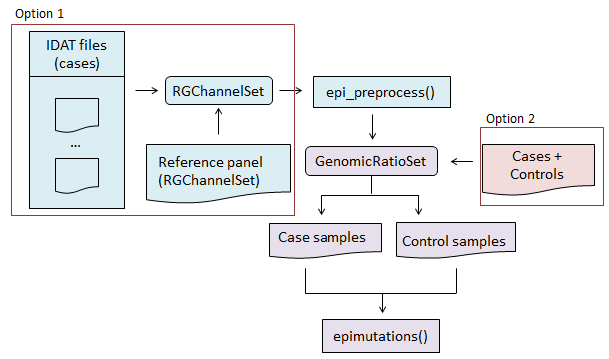
\includegraphics[width=0.9\linewidth]{C:/Users/nla94/Documents/GitHub/Supplementary-Material/Abarrategui_2021/vignette/fig/workflow} 

}

\caption{Allowed data formats, normalization and input types}\label{fig:workflow}
\end{figure}

\hypertarget{getting-started}{%
\section{Getting started}\label{getting-started}}

The \texttt{epimutacions} package is installed by executing:

\begin{Shaded}
\begin{Highlighting}[]
\KeywordTok{install_github}\NormalTok{(}\StringTok{"isglobal-brge/epimutacions"}\NormalTok{)}
\end{Highlighting}
\end{Shaded}

The package is it loaded in R as usual:

\begin{Shaded}
\begin{Highlighting}[]
\KeywordTok{library}\NormalTok{(epimutacions)}
\end{Highlighting}
\end{Shaded}

The document has the following dependencies:

\begin{Shaded}
\begin{Highlighting}[]
\KeywordTok{library}\NormalTok{(Knitr)}
\KeywordTok{library}\NormalTok{(kableExtra)}
\end{Highlighting}
\end{Shaded}

\hypertarget{datasets}{%
\section{Datasets}\label{datasets}}

\hypertarget{candidate-regions}{%
\subsection{Candidate regions}\label{candidate-regions}}

Epimutations detection has two main steps: (1) definition of candidate
regions and (2) evaluation of outlier significance. Although there are
different algorithms to define epimutations regions, they share common
features. In general, we define an epimutation as at least 3 contiguous
CpGs with a maximum distance of 1kb between them.

In Illumina 450K array, probes are unequally distributed along the
genome, limiting the number of regions that can fulfil the requirements
to be considered an epimutation. So, we have computed a dataset
containing the regions that are candidates to become an epimutation.

To define the candidate epimutations, we relied on the clustering from
bumphunter. We defined a primary dataset with all the CpGs from the
Illumina 450K array. Then, we run bumphunter and selected those regions
with at least 3 CpGs. As a result, we found 40408 candidate epimutations
which are available in \texttt{candRegsGR} dataset. The code for
generating these regions can be found in epimutacion package.

In addition, we converted the candidate region from hg19 to hg38
coordinates, using NCBI remap. We selected regions that mapped to one
region in hg38 with the same length. This yielded a total of 39944, the
98.85\% of total hg19 regions. After converting to hg38, we can use
these ranges to be annotated to ENCODE cREs. Overall, we mapped 30163
candidate regions to cREs, representing 74.65\% of total candidate
regions.

\begin{Shaded}
\begin{Highlighting}[]
\KeywordTok{data}\NormalTok{(}\StringTok{"candRegsGR"}\NormalTok{)}
\NormalTok{candRegsGR}
\end{Highlighting}
\end{Shaded}

\begin{verbatim}
GRanges object with 40408 ranges and 9 metadata columns:
                 seqnames              ranges strand |     value      area
                    <Rle>           <IRanges>  <Rle> | <numeric> <numeric>
   chr6_32128101     chr6   32128101-32173532      * |         1       381
   chr6_33156164     chr6   33156164-33181870      * |         1       291
   chr6_32034322     chr6   32034322-32059605      * |         1       239
   chr6_31618987     chr6   31618987-31639143      * |         1       234
   chr6_33279563     chr6   33279563-33292029      * |         1       233
             ...      ...                 ...    ... .       ...       ...
  chr9_140652685     chr9 140652685-140652743      * |         1         3
  chr9_140656200     chr9 140656200-140657381      * |         1         3
  chr9_140680393     chr9 140680393-140681206      * |         1         3
  chr9_140732731     chr9 140732731-140733980      * |         1         3
  chr9_141012312     chr9 141012312-141013537      * |         1         3
                   cluster indexStart  indexEnd         L  clusterL
                 <numeric>  <integer> <integer> <numeric> <integer>
   chr6_32128101    133070     165174    165554       381       381
   chr6_33156164    133204     167451    167741       291       291
   chr6_32034322    133058     164512    164750       239       239
   chr6_31618987    132987     162583    162816       234       234
   chr6_33279563    133221     168282    168514       233       233
             ...       ...        ...       ...       ...       ...
  chr9_140652685    162642     247198    247200         3         3
  chr9_140656200    162643     247201    247203         3         3
  chr9_140680393    162649     247214    247216         3         3
  chr9_140732731    162660     247252    247254         3         3
  chr9_141012312    162683     247294    247296         3         3
                                    CRE               CRE_type
                            <character>            <character>
   chr6_32128101 EH38E2459822,EH38E24.. pELS,CTCF-bound;PLS;..
   chr6_33156164 EH38E2460436,EH38E24.. PLS;pELS,CTCF-bound;..
   chr6_32034322 EH38E2459711,EH38E24.. dELS;dELS;dELS;pELS,..
   chr6_31618987 EH38E2459340,EH38E24.. pELS,CTCF-bound;PLS,..
   chr6_33279563 EH38E2460551,EH38E24.. pELS,CTCF-bound;pELS..
             ...                    ...                    ...
  chr9_140652685                                              
  chr9_140656200 EH38E2738315,EH38E27.. pELS,CTCF-bound;pELS..
  chr9_140680393 EH38E2738332,EH38E27..   dELS,CTCF-bound;dELS
  chr9_140732731                                              
  chr9_141012312                                              
  -------
  seqinfo: 22 sequences from an unspecified genome; no seqlengths
\end{verbatim}

\hypertarget{genomicratioset}{%
\subsection{GenomicRatioSet}\label{genomicratioset}}

The package includes a small \texttt{GenomicRatioSet} class dataset
(\texttt{methy} ) containing the DNA methylation profiles from a total
of individuals, 3 cases and 48 controls. The DNA methylation profiles
were generated using the Illumina 450k Human Methylation BeadChip. The
data were obtained from \href{https://www.ncbi.nlm.nih.gov/geo/}{Gene
Expression Omnibus (GEO)} and adapted for the package usage.

\begin{Shaded}
\begin{Highlighting}[]
\KeywordTok{data}\NormalTok{(}\StringTok{"methy"}\NormalTok{)}
\NormalTok{methy}
\end{Highlighting}
\end{Shaded}

\begin{verbatim}
class: GenomicRatioSet 
dim: 80731 51 
metadata(0):
assays(3): Beta M CN
rownames(80731): cg00725145 cg16080333 ... cg07468397 cg08821909
rowData names(0):
colnames(51): GSM2808239 GSM2808240 ... GSM2562700 GSM2562701
colData names(4): sampleID age sex status
Annotation
  array: IlluminaHumanMethylation450k
  annotation: ilmn12.hg19
Preprocessing
  Method: NA
  minfi version: NA
  Manifest version: NA
\end{verbatim}

\begin{Shaded}
\begin{Highlighting}[]
\KeywordTok{table}\NormalTok{(methy}\OperatorTok{$}\NormalTok{status)}
\end{Highlighting}
\end{Shaded}

\begin{verbatim}

   case control 
      3      48 
\end{verbatim}

We are going to create two different datasets for further analysis,
\texttt{case\_samples} and \texttt{control\_panel}:

\begin{Shaded}
\begin{Highlighting}[]
\NormalTok{case_samples <-}\StringTok{ }\NormalTok{methy[,methy}\OperatorTok{$}\NormalTok{status }\OperatorTok{==}\StringTok{ "case"}\NormalTok{]}
\NormalTok{control_samples <-}\StringTok{ }\NormalTok{methy[,methy}\OperatorTok{$}\NormalTok{status }\OperatorTok{==}\StringTok{ "control"}\NormalTok{]}
\end{Highlighting}
\end{Shaded}

\hypertarget{preprocessing}{%
\section{Preprocessing}\label{preprocessing}}

The preprocessing in \texttt{epimutacions} package is done by
\texttt{epi\_preprocess()} function. It contains 6 preprocessing methods
corresponding to minfi package that can be selected by the user:

\begin{longtable}[]{@{}lll@{}}
\toprule
\begin{minipage}[b]{0.12\columnwidth}\raggedright
Method\strut
\end{minipage} & \begin{minipage}[b]{0.23\columnwidth}\raggedright
Function\strut
\end{minipage} & \begin{minipage}[b]{0.55\columnwidth}\raggedright
Description\strut
\end{minipage}\tabularnewline
\midrule
\endhead
\begin{minipage}[t]{0.12\columnwidth}\raggedright
\texttt{raw}\strut
\end{minipage} & \begin{minipage}[t]{0.23\columnwidth}\raggedright
\texttt{preprocessRaw}\strut
\end{minipage} & \begin{minipage}[t]{0.55\columnwidth}\raggedright
Converts the Red/Green channel for an Illumina methylation array into
methylation signal, without using any normalization\strut
\end{minipage}\tabularnewline
\begin{minipage}[t]{0.12\columnwidth}\raggedright
\texttt{illumina}\strut
\end{minipage} & \begin{minipage}[t]{0.23\columnwidth}\raggedright
\texttt{preprocessIllumina}\strut
\end{minipage} & \begin{minipage}[t]{0.55\columnwidth}\raggedright
Implements preprocessing for Illumina methylation microarrays as used in
Genome Studio\strut
\end{minipage}\tabularnewline
\begin{minipage}[t]{0.12\columnwidth}\raggedright
\texttt{swan}\strut
\end{minipage} & \begin{minipage}[t]{0.23\columnwidth}\raggedright
\texttt{preprocessSWAN}\strut
\end{minipage} & \begin{minipage}[t]{0.55\columnwidth}\raggedright
Subset-quantile Within Array Normalisation (SWAN). It allows Infinium I
and II type probes on a single array to be normalized together\strut
\end{minipage}\tabularnewline
\begin{minipage}[t]{0.12\columnwidth}\raggedright
\texttt{quantile}\strut
\end{minipage} & \begin{minipage}[t]{0.23\columnwidth}\raggedright
\texttt{preprocessQuantile}\strut
\end{minipage} & \begin{minipage}[t]{0.55\columnwidth}\raggedright
Implements stratified quantile normalization preprocessing for Illumina
methylation microarrays\strut
\end{minipage}\tabularnewline
\begin{minipage}[t]{0.12\columnwidth}\raggedright
\texttt{noob}\strut
\end{minipage} & \begin{minipage}[t]{0.23\columnwidth}\raggedright
\texttt{preprocessNoob}\strut
\end{minipage} & \begin{minipage}[t]{0.55\columnwidth}\raggedright
Noob (normal-exponential out-of-band) is a background correction method
with dye-bias normalization for Illumina Infinium methylation
arrays\strut
\end{minipage}\tabularnewline
\begin{minipage}[t]{0.12\columnwidth}\raggedright
\texttt{funnorm}\strut
\end{minipage} & \begin{minipage}[t]{0.23\columnwidth}\raggedright
\texttt{preprocessFunnorm}\strut
\end{minipage} & \begin{minipage}[t]{0.55\columnwidth}\raggedright
Functional normalization (FunNorm) is a between-array normalization
method for the Illumina Infinium HumanMethylation450 platform\strut
\end{minipage}\tabularnewline
\bottomrule
\end{longtable}

In addition, the unique parameters for each normalization approach are
defined through \texttt{norm\_parameters()}:

\begin{longtable}[]{@{}lll@{}}
\toprule
\begin{minipage}[b]{0.09\columnwidth}\raggedright
Method\strut
\end{minipage} & \begin{minipage}[b]{0.19\columnwidth}\raggedright
Parameters\strut
\end{minipage} & \begin{minipage}[b]{0.63\columnwidth}\raggedright
Description\strut
\end{minipage}\tabularnewline
\midrule
\endhead
\begin{minipage}[t]{0.09\columnwidth}\raggedright
\texttt{illumina}\strut
\end{minipage} & \begin{minipage}[t]{0.19\columnwidth}\raggedright
\texttt{bg.correct}~\\
\texttt{normalize}~\\
\texttt{reference}\strut
\end{minipage} & \begin{minipage}[t]{0.63\columnwidth}\raggedright
Performs background correction\\
Performs controls normalization\\
The reference array for control normalization\strut
\end{minipage}\tabularnewline
\begin{minipage}[t]{0.09\columnwidth}\raggedright
\texttt{quantile}\strut
\end{minipage} & \begin{minipage}[t]{0.19\columnwidth}\raggedright
\texttt{fixOutliers}~\\
\texttt{removeBadSamples}~\\
\texttt{badSampleCutoff}~\\
\texttt{quantileNormalize}~\\
\texttt{stratified} \texttt{mergeManifest}~\\
~\\
\texttt{sex}\strut
\end{minipage} & \begin{minipage}[t]{0.63\columnwidth}\raggedright
Low outlier Meth and Unmeth signals will be fixed\\
Remove bad samples\\
The cutoff to label samples as `bad'\\
Performs quantile normalization\\
Performs quantile normalization within region strata\\
Merged to the output the information in the associated manifest
package\\

Sex of the samples\strut
\end{minipage}\tabularnewline
\begin{minipage}[t]{0.09\columnwidth}\raggedright
\texttt{noob}\strut
\end{minipage} & \begin{minipage}[t]{0.19\columnwidth}\raggedright
\texttt{offset}~\\
\texttt{dyeCorr}~\\
\texttt{dyeMethod}\strut
\end{minipage} & \begin{minipage}[t]{0.63\columnwidth}\raggedright
Offset for the normexp background correct\\
Performs dye normalization\\
Dye bias correction to be done\strut
\end{minipage}\tabularnewline
\begin{minipage}[t]{0.09\columnwidth}\raggedright
\texttt{funnorm}\strut
\end{minipage} & \begin{minipage}[t]{0.19\columnwidth}\raggedright
\texttt{nPCs}~\\
\texttt{sex}~\\
\texttt{bgCorr}~\\
~\\
\texttt{dyeCorr}~\\
\texttt{keepCN}\strut
\end{minipage} & \begin{minipage}[t]{0.63\columnwidth}\raggedright
The number of principal components from the control probes\\
Sex of the samples\\
Performs NOOB background correction prior to functional normalization\\

Performs dye normalization\\
Keeps copy number estimates\strut
\end{minipage}\tabularnewline
\bottomrule
\end{longtable}

The default settings for each method can be obtained by invoking the
function \texttt{norm\_parameters()} with no arguments:

\begin{Shaded}
\begin{Highlighting}[]
\KeywordTok{norm_parameters}\NormalTok{()}
\end{Highlighting}
\end{Shaded}

\begin{verbatim}
$illumina
$illumina$bg.correct
[1] TRUE

$illumina$normalize
[1] "controls" "no"      

$illumina$reference
[1] 1


$quantile
$quantile$fixOutliers
[1] TRUE

$quantile$removeBadSamples
[1] FALSE

$quantile$badSampleCutoff
[1] 10.5

$quantile$quantileNormalize
[1] TRUE

$quantile$stratified
[1] TRUE

$quantile$mergeManifest
[1] FALSE

$quantile$sex
NULL


$noob
$noob$offset
[1] 15

$noob$dyeCorr
[1] TRUE

$noob$dyeMethod
[1] "single"    "reference"


$funnorm
$funnorm$nPCs
[1] 2

$funnorm$sex
NULL

$funnorm$bgCorr
[1] TRUE

$funnorm$dyeCorr
[1] TRUE

$funnorm$keepCN
[1] FALSE
\end{verbatim}

However, to modify the parameters related to a method you can do as the
following example for \texttt{illumina} approach:

\begin{Shaded}
\begin{Highlighting}[]
\NormalTok{parameters <-}\StringTok{ }\KeywordTok{norm_parameters}\NormalTok{(}\DataTypeTok{illumina =} \KeywordTok{list}\NormalTok{(}\StringTok{"bg.correct"}\NormalTok{ =}\StringTok{ }\OtherTok{FALSE}\NormalTok{))}
\NormalTok{parameters}\OperatorTok{$}\NormalTok{illumina}\OperatorTok{$}\NormalTok{bg.correct}
\end{Highlighting}
\end{Shaded}

\begin{verbatim}
[1] FALSE
\end{verbatim}

\hypertarget{epimutations}{%
\section{Epimutations}\label{epimutations}}

\hypertarget{epimutations-detection}{%
\subsection{Epimutations detection}\label{epimutations-detection}}

The \texttt{epimutacions} package includes 6 methods for epivariants
identification: (1) Multivariate Analysis of variance (\texttt{manova}),
(2) Multivariate Linear Model (\texttt{mlm}), (3) isolation forest
(\texttt{isoforest}), (4) robust mahalanobis distance
(\texttt{mahdistmcd}) (5) \texttt{barbosa} and (6) \texttt{beta}.

In the mentioned first 4 methods, firstly, Differentially Methylated
Regions (DMRs) are identified using bump-hunter method (Jaffe et al.
2012). Then, those DMRs are tested to identify regions with CpGs being
outliers when comparing with the reference panel. However,
\texttt{barbosa} and \texttt{beta} do not identify outliers by filtering
the DMRs. \texttt{barbosa} utilized a sliding window approach to
individually compare the methylation value in each proband against the
reference panel. \texttt{Beta} used beta distribution to identify
epivariants in the case sample.

\begin{Shaded}
\begin{Highlighting}[]
\NormalTok{epi_mvo <-}\StringTok{ }\KeywordTok{epimutations}\NormalTok{(case_samples, control_samples, }\DataTypeTok{method =} \StringTok{"manova"}\NormalTok{)}
\NormalTok{epi_ml <-}\StringTok{ }\KeywordTok{epimutations}\NormalTok{(case_samples, control_samples, }\DataTypeTok{method =} \StringTok{"mlm"}\NormalTok{)}
\NormalTok{epi_iso <-}\StringTok{ }\KeywordTok{epimutations}\NormalTok{(case_samples, control_samples, }\DataTypeTok{method =} \StringTok{"isoforest"}\NormalTok{)}
\NormalTok{epi_mcd <-}\StringTok{ }\KeywordTok{epimutations}\NormalTok{(case_samples, control_samples, }\DataTypeTok{method =} \StringTok{"mahdistmcd"}\NormalTok{)}
\end{Highlighting}
\end{Shaded}

\begin{Shaded}
\begin{Highlighting}[]
\NormalTok{epi_brb <-}\StringTok{ }\KeywordTok{epimutations}\NormalTok{(case_samples, control_samples, }\DataTypeTok{method =} \StringTok{"barbosa"}\NormalTok{)}
\NormalTok{epi_beta <-}\StringTok{ }\KeywordTok{epimutations}\NormalTok{(case_samples, control_samples, }\DataTypeTok{method =} \StringTok{"beta"}\NormalTok{)}
\end{Highlighting}
\end{Shaded}

\hypertarget{unique-parameters}{%
\subsection{Unique parameters}\label{unique-parameters}}

The \texttt{epi\_parameters()} function is useful to set the individual
parameters for each approach. The arguments are described in the
following table:

\begin{longtable}[]{@{}lll@{}}
\toprule
\begin{minipage}[b]{0.12\columnwidth}\raggedright
Method\strut
\end{minipage} & \begin{minipage}[b]{0.23\columnwidth}\raggedright
Parameter\strut
\end{minipage} & \begin{minipage}[b]{0.55\columnwidth}\raggedright
Description\strut
\end{minipage}\tabularnewline
\midrule
\endhead
\begin{minipage}[t]{0.12\columnwidth}\raggedright
\texttt{manova}~\\
\texttt{mlm}~\\
\texttt{beta}\strut
\end{minipage} & \begin{minipage}[t]{0.23\columnwidth}\raggedright
\texttt{pvalue\_cutoff}\strut
\end{minipage} & \begin{minipage}[t]{0.55\columnwidth}\raggedright
The threshold p-value to select which CpG regions are outliers\strut
\end{minipage}\tabularnewline
\begin{minipage}[t]{0.12\columnwidth}\raggedright
\texttt{iso.forest}\strut
\end{minipage} & \begin{minipage}[t]{0.23\columnwidth}\raggedright
\texttt{outlier\_score\_cutoff}~\\
\texttt{ntrees}\strut
\end{minipage} & \begin{minipage}[t]{0.55\columnwidth}\raggedright
The threshold to select which CpG regions are outliers\\
The number of binary trees to build for the model\strut
\end{minipage}\tabularnewline
\begin{minipage}[t]{0.12\columnwidth}\raggedright
\texttt{mahdist.mcd}\strut
\end{minipage} & \begin{minipage}[t]{0.23\columnwidth}\raggedright
\texttt{nsamp}\strut
\end{minipage} & \begin{minipage}[t]{0.55\columnwidth}\raggedright
The number of subsets used for initial estimates in the MCD\strut
\end{minipage}\tabularnewline
\begin{minipage}[t]{0.12\columnwidth}\raggedright
\texttt{barbosa}\strut
\end{minipage} & \begin{minipage}[t]{0.23\columnwidth}\raggedright
\texttt{window\_sz}~\\
~\\
\texttt{offset\_mean}/\texttt{offset\_abs}\strut
\end{minipage} & \begin{minipage}[t]{0.55\columnwidth}\raggedright
The maximum distance between CpGs to be considered in the same DMR\\

The upper and lower threshold to consider a CpG an outlier\strut
\end{minipage}\tabularnewline
\begin{minipage}[t]{0.12\columnwidth}\raggedright
\texttt{beta}\strut
\end{minipage} & \begin{minipage}[t]{0.23\columnwidth}\raggedright
\texttt{pvalue\_cutoff}~\\
\texttt{diff\_threshold}\strut
\end{minipage} & \begin{minipage}[t]{0.55\columnwidth}\raggedright
The minimum p-value to consider a CpG an outlier\\
The minimum methylation difference between the CpG and the mean
methylation to consider a position an outlier\strut
\end{minipage}\tabularnewline
\bottomrule
\end{longtable}

Invoking \texttt{epi\_parameters()} with no arguments returns a list of
the default settings for each method:

\begin{Shaded}
\begin{Highlighting}[]
\KeywordTok{epi_parameters}\NormalTok{()}
\end{Highlighting}
\end{Shaded}

\begin{verbatim}
$manova
$manova$pvalue_cutoff
[1] 0.05


$mlm
$mlm$pvalue_cutoff
[1] 0.05


$isoforest
$isoforest$outlier_score_cutoff
[1] 0.5

$isoforest$ntrees
[1] 100


$mahdistmcd
$mahdistmcd$nsamp
[1] "deterministic"


$barbosa
$barbosa$window_sz
[1] 10

$barbosa$offset_mean
[1] 0.15

$barbosa$offset_abs
[1] 0.1


$beta
$beta$pvalue_cutoff
[1] 1e-06

$beta$diff_threshold
[1] 0.1
\end{verbatim}

The set up of any parameter can be done as the following example of
p-value cut-off for \texttt{manova}:

\begin{Shaded}
\begin{Highlighting}[]
\NormalTok{parameters <-}\StringTok{ }\KeywordTok{epi_parameters}\NormalTok{(}\DataTypeTok{manova =} \KeywordTok{list}\NormalTok{(}\StringTok{"pvalue_cutoff"}\NormalTok{ =}\StringTok{ }\FloatTok{0.01}\NormalTok{))}
\NormalTok{parameters}\OperatorTok{$}\NormalTok{manova}\OperatorTok{$}\NormalTok{pvalue_cutoff}
\end{Highlighting}
\end{Shaded}

\begin{verbatim}
[1] 0.01
\end{verbatim}

\hypertarget{results-description}{%
\subsection{Results description}\label{results-description}}

The \texttt{epimutations} function returns a tibble containing all the
epivariants identified in the given case sample. In case no epimutation
is found, a row containing the case sample information and missing
values for each argument is returned. The following table describes each
argument in the result data frame:

\begin{longtable}[]{@{}ll@{}}
\toprule
\begin{minipage}[b]{0.16\columnwidth}\raggedright
Column name\strut
\end{minipage} & \begin{minipage}[b]{0.78\columnwidth}\raggedright
Description\strut
\end{minipage}\tabularnewline
\midrule
\endhead
\begin{minipage}[t]{0.16\columnwidth}\raggedright
\texttt{epi\_id}\strut
\end{minipage} & \begin{minipage}[t]{0.78\columnwidth}\raggedright
Systematic name for each epimutation identified\strut
\end{minipage}\tabularnewline
\begin{minipage}[t]{0.16\columnwidth}\raggedright
\texttt{sample}\strut
\end{minipage} & \begin{minipage}[t]{0.78\columnwidth}\raggedright
The name of the sample containing that epimutation\strut
\end{minipage}\tabularnewline
\begin{minipage}[t]{0.16\columnwidth}\raggedright
\texttt{chromosome} \texttt{start} \texttt{end}\strut
\end{minipage} & \begin{minipage}[t]{0.78\columnwidth}\raggedright
The location of the epimutation\strut
\end{minipage}\tabularnewline
\begin{minipage}[t]{0.16\columnwidth}\raggedright
\texttt{sz}\strut
\end{minipage} & \begin{minipage}[t]{0.78\columnwidth}\raggedright
The window's size of the event\strut
\end{minipage}\tabularnewline
\begin{minipage}[t]{0.16\columnwidth}\raggedright
\texttt{cpg\_n}\strut
\end{minipage} & \begin{minipage}[t]{0.78\columnwidth}\raggedright
The number of CpGs in the epimutation\strut
\end{minipage}\tabularnewline
\begin{minipage}[t]{0.16\columnwidth}\raggedright
\texttt{cpg\_n}\strut
\end{minipage} & \begin{minipage}[t]{0.78\columnwidth}\raggedright
The names of CpGs in the epimutation\strut
\end{minipage}\tabularnewline
\begin{minipage}[t]{0.16\columnwidth}\raggedright
\texttt{outlier\_score}\strut
\end{minipage} & \begin{minipage}[t]{0.78\columnwidth}\raggedright
For method \texttt{manova} it provides the approximation to F-test and
the Pillai score, separated by \texttt{/}\\
For method \texttt{mlm} it provides the approximation to F-test and the
R2 of the model, separated by \texttt{/}\\
For method \texttt{isoforest} it provides the magnitude of the outlier
score.\\
For method \texttt{beta} it provides the mean p-value of all GpGs in
that DMR\\
For methods \texttt{barbosa} and \texttt{mahdistmcd} it is filled with
\texttt{NA}.\strut
\end{minipage}\tabularnewline
\begin{minipage}[t]{0.16\columnwidth}\raggedright
\texttt{pvalue}\strut
\end{minipage} & \begin{minipage}[t]{0.78\columnwidth}\raggedright
For methods \texttt{manova} and \texttt{mlm} it provides the p-value
obtained from the model.\\
For method \texttt{barbosa}, \texttt{isoforest}, \texttt{beta} and
\texttt{mahdistmcd} it is filled with \texttt{NA}.\strut
\end{minipage}\tabularnewline
\begin{minipage}[t]{0.16\columnwidth}\raggedright
\texttt{outlier\_direction}\strut
\end{minipage} & \begin{minipage}[t]{0.78\columnwidth}\raggedright
Indicates the direction of the outlier with ``hypomethylation'' and
``hypermethylation''.\\
For \texttt{manova}, \texttt{mlm}, \texttt{isoforest}, and
\texttt{mahdistmcd} it is computed from the values obtained from
\texttt{bumphunter}.\\
For \texttt{beta} is computed from the p value for each CpG using
\texttt{diff\_threshold} and \texttt{pvalue\_threshold} arguments.\\
For \texttt{barbosa} it is computed from the location of the sample in
the reference distribution (left vs.~right outlier).\strut
\end{minipage}\tabularnewline
\begin{minipage}[t]{0.16\columnwidth}\raggedright
\texttt{adj\_pvalue}\strut
\end{minipage} & \begin{minipage}[t]{0.78\columnwidth}\raggedright
For methods \texttt{manova} and \texttt{mlm} it provides the adjusted
p-value with Benjamini-Hochberg based on the total number of regions
detected by Bumphunter.\\
For method \texttt{barbosa}, \texttt{isoforest}, \texttt{mahdistmcd} and
\texttt{beta} it is filled with \texttt{NA}.\strut
\end{minipage}\tabularnewline
\begin{minipage}[t]{0.16\columnwidth}\raggedright
\texttt{epi\_region\_id}\strut
\end{minipage} & \begin{minipage}[t]{0.78\columnwidth}\raggedright
Name of the epimutation region as defined in \texttt{candRegsGR}.\strut
\end{minipage}\tabularnewline
\begin{minipage}[t]{0.16\columnwidth}\raggedright
\texttt{CRE}\strut
\end{minipage} & \begin{minipage}[t]{0.78\columnwidth}\raggedright
cREs (cis-Regulatory Elements) as defined by ENCODE overlapping the
epimutation region.\strut
\end{minipage}\tabularnewline
\begin{minipage}[t]{0.16\columnwidth}\raggedright
\texttt{CRE\_type}\strut
\end{minipage} & \begin{minipage}[t]{0.78\columnwidth}\raggedright
Type of cREs (cis-Regulatory Elements) as defined by ENCODE.\strut
\end{minipage}\tabularnewline
\bottomrule
\end{longtable}

\hypertarget{epimutations-annotations}{%
\subsection{Epimutations annotations}\label{epimutations-annotations}}

The \texttt{epimutacions} package also includes the
\texttt{annotate\_epimutations} function dedicated to enriching the
epimutations identified by the previously described methods:

\begin{Shaded}
\begin{Highlighting}[]
\NormalTok{rst_mvo <-}\StringTok{ }\KeywordTok{annotate_epimutations}\NormalTok{(epi_mvo)}
\end{Highlighting}
\end{Shaded}

\begin{Shaded}
\begin{Highlighting}[]
\NormalTok{rst_mvo[}\DecValTok{1}\OperatorTok{:}\DecValTok{2}\NormalTok{, }\KeywordTok{c}\NormalTok{(}\DecValTok{1}\NormalTok{, }\DecValTok{12}\OperatorTok{:}\DecValTok{14}\NormalTok{)]}
\end{Highlighting}
\end{Shaded}

\begin{longtable}[]{@{}lrll@{}}
\caption{epimutations annotation}\tabularnewline
\toprule
\begin{minipage}[b]{0.06\columnwidth}\raggedright
epi\_id\strut
\end{minipage} & \begin{minipage}[b]{0.05\columnwidth}\raggedleft
adj\_pvalue\strut
\end{minipage} & \begin{minipage}[b]{0.07\columnwidth}\raggedright
epi\_region\_id\strut
\end{minipage} & \begin{minipage}[b]{0.70\columnwidth}\raggedright
CRE\strut
\end{minipage}\tabularnewline
\midrule
\endfirsthead
\toprule
\begin{minipage}[b]{0.06\columnwidth}\raggedright
epi\_id\strut
\end{minipage} & \begin{minipage}[b]{0.05\columnwidth}\raggedleft
adj\_pvalue\strut
\end{minipage} & \begin{minipage}[b]{0.07\columnwidth}\raggedright
epi\_region\_id\strut
\end{minipage} & \begin{minipage}[b]{0.70\columnwidth}\raggedright
CRE\strut
\end{minipage}\tabularnewline
\midrule
\endhead
\begin{minipage}[t]{0.06\columnwidth}\raggedright
epi\_manova\_1\strut
\end{minipage} & \begin{minipage}[t]{0.05\columnwidth}\raggedleft
0\strut
\end{minipage} & \begin{minipage}[t]{0.07\columnwidth}\raggedright
chr19\_12776725\strut
\end{minipage} & \begin{minipage}[t]{0.70\columnwidth}\raggedright
EH38E1939817,EH38E1939818,EH38E1939819\strut
\end{minipage}\tabularnewline
\begin{minipage}[t]{0.06\columnwidth}\raggedright
epi\_manova\_2\strut
\end{minipage} & \begin{minipage}[t]{0.05\columnwidth}\raggedleft
0\strut
\end{minipage} & \begin{minipage}[t]{0.07\columnwidth}\raggedright
chr7\_90892836\strut
\end{minipage} & \begin{minipage}[t]{0.70\columnwidth}\raggedright
EH38E2570884,EH38E2570885,EH38E2570886,EH38E2570887,EH38E2570888,EH38E2570889,EH38E2570890,EH38E2570891,EH38E2570892,EH38E2570893,EH38E2570894\strut
\end{minipage}\tabularnewline
\bottomrule
\end{longtable}

\hypertarget{epimutation-visualization}{%
\subsection{Epimutation visualization}\label{epimutation-visualization}}

The visualization approach locates the epimutations along the genome.
The function \texttt{plot\_epimutations} plots the methylation values of
the individual with the epimutation in red, the control samples in
dashed black lines and population mean in blue:

\begin{Shaded}
\begin{Highlighting}[]
\KeywordTok{plot_epimutations}\NormalTok{(}\KeywordTok{as.data.frame}\NormalTok{(epi_mvo[}\DecValTok{1}\NormalTok{,]), methy)}
\end{Highlighting}
\end{Shaded}

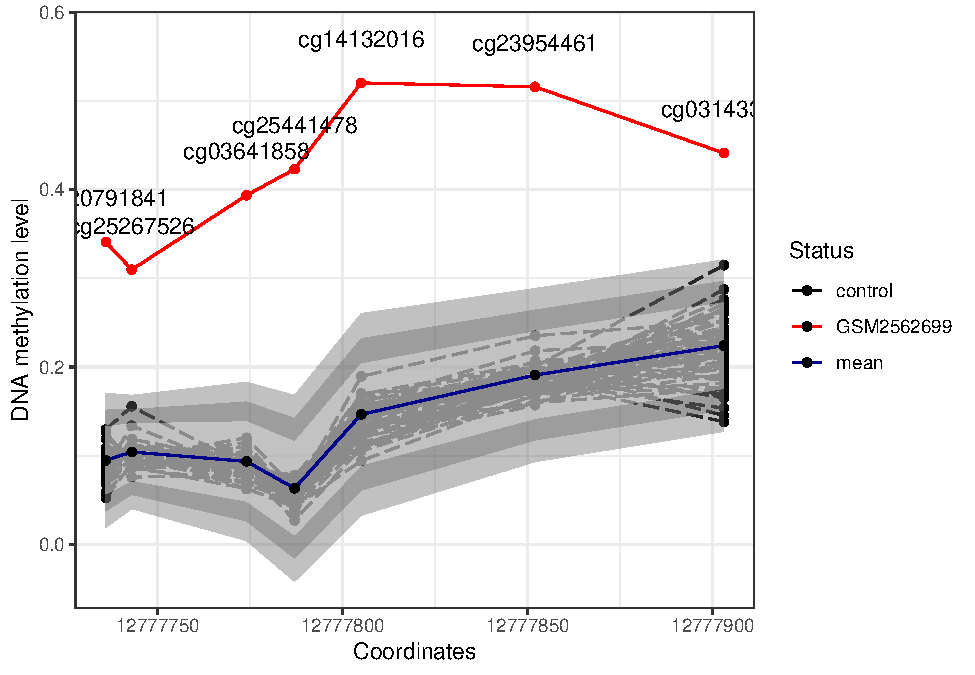
\includegraphics{sup_mat_files/figure-latex/unnamed-chunk-12-1.pdf}

Furthermore, it includes the gene annotations in the regions in which
the epivariation is located. This can be achieved by using the argument
\texttt{gene\_annot\ ==\ TRUE}:

\begin{Shaded}
\begin{Highlighting}[]
\KeywordTok{plot_epimutations}\NormalTok{(}\KeywordTok{as.data.frame}\NormalTok{(epi_mvo[}\DecValTok{1}\NormalTok{,]), methy, }\DataTypeTok{genes_annot =} \OtherTok{TRUE}\NormalTok{)}
\end{Highlighting}
\end{Shaded}

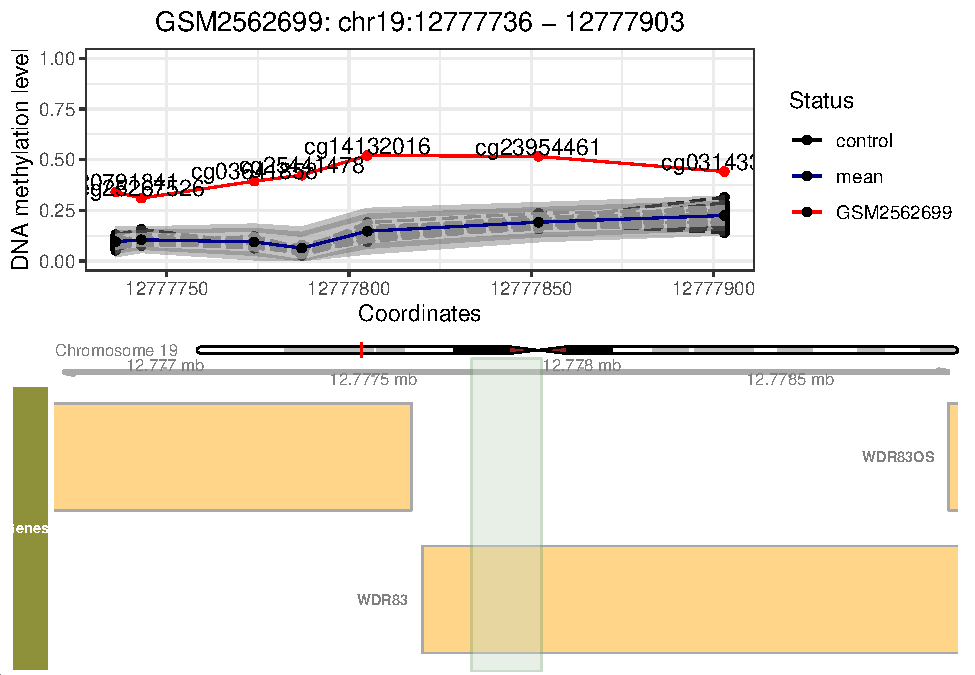
\includegraphics{sup_mat_files/figure-latex/plot_mvo_genes_annot-1.pdf}

Also, it is possible to plot the chromatin marks H3K4me3, H3K27me3 and
H3K27ac by setting the argument \texttt{regulation\ =\ TRUE}:

\begin{itemize}
\tightlist
\item
  \textbf{H3K4me3}: commonly associated with the activation of
  transcription of nearby genes.
\item
  \textbf{H3K27me3}: is used in epigenetics to look for inactive genes.
\item
  \textbf{H3K27ac}: is associated with the higher activation of
  transcription and therefore defined as an active enhancer mark
\end{itemize}

\begin{Shaded}
\begin{Highlighting}[]
\KeywordTok{plot_epimutations}\NormalTok{(}\KeywordTok{as.data.frame}\NormalTok{(epi_mvo[}\DecValTok{1}\NormalTok{,]), methy, }\DataTypeTok{regulation =} \OtherTok{TRUE}\NormalTok{)}
\end{Highlighting}
\end{Shaded}

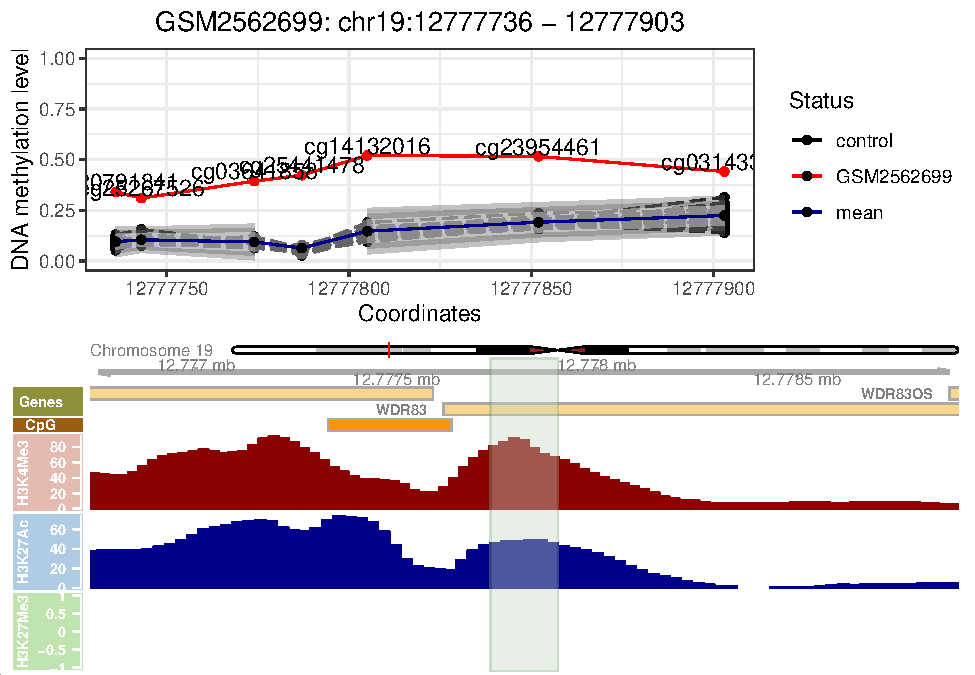
\includegraphics{sup_mat_files/figure-latex/plot_mvo_regulation-1.pdf}

\hypertarget{method-validation}{%
\section{Method validation}\label{method-validation}}

\hypertarget{data-collection}{%
\subsection{Data collection}\label{data-collection}}

The data were obtained for the studies previously described (Garg et al.
2020). The datasets were downloaded from
\href{https://www.ncbi.nlm.nih.gov/geo/}{Gene Expression Omnibus (GEO)}.
We accessed DNA methylation data from a total 1, 417 individuals from
\href{https://www.ncbi.nlm.nih.gov/geo/query/acc.cgi?acc=GSE51032}{GSE51032}
and \href{https://www.ncbi.nlm.nih.gov/geo/query/acc.cgi}{GSE111629}
cohorts. The DNA methylation profiles were generated using the Illumina
450k Human Methylation BeadChip.

The GSE51032 study analysed primary cancers samples: 424 cancer free,
235 primary breast cancer, 166 primary colorectal cancer and 20 other
primary cancers. The GSE111629 cohort 335 Parkinson's disease and 237
control samples.

\hypertarget{validation}{%
\subsection{Validation}\label{validation}}

We evaluated the performance of the method using TPR (True Positive
Rate), False Positive Rate (FPR) and accuracy. We use the TPR to measure
the proportion of detected epivariations by the \texttt{epimutations}
approach present in the validated (Garg et al. 2020). FPR to calculate
the identified epimutations outside the once found in (Garg et al.
2020), whether validated or not. The accuracy measures the closeness of
the detected epimutation to the validated regions.

We select samples differently depending on the study group and measure
to compute. Control samples were selected randomly using different
sample size: 20, 30, 40, 50, 60, 70, 80, 90 and 100. However, case
samples were selected considering validated epimutations (for TPR and
accuracy) or excluding epivariations found (for FPR) (Garg et al. 2020).

The validated epimutations in table 1 were only present on 5
individuals: GSM1235784 from GSE51032 cohort and GSM3035933, GSM3035791,
GSM3035807 and GSM3035685 from GSE111629. Therefore, they were
established as case samples when computing TPR and accuracy.
Nevertheless, we compute FPR excluding the samples containing at least
one epimutation found by (Garg et al. 2020). For the remaining case
samples, 4 were selected randomly in each execution.

We execute 100 times the same process for each control sample size. We
define for the analysis regions of \(\approx\) 20 kb containing \(\ge\)
3 GpGs.

\begin{longtable}[]{@{}lrrrll@{}}
\caption{validated epimutations (Garg et al.~2020).}\tabularnewline
\toprule
Chromosome & Start & End & Width & Strand & Samples\tabularnewline
\midrule
\endfirsthead
\toprule
Chromosome & Start & End & Width & Strand & Samples\tabularnewline
\midrule
\endhead
chr17 & 46018653 & 46019185 & 533 & * &
GSM1235784/GSM3035791\tabularnewline
chr19 & 11199850 & 11200147 & 298 & * & GSM3035685\tabularnewline
chr5 & 10249760 & 10251253 & 1494 & * & GSM3035933\tabularnewline
chr5 & 67583971 & 67584381 & 411 & * &
GSM3035791/GSM3035807\tabularnewline
\bottomrule
\end{longtable}

Additionally, we have plotted the methylation values of the samples in
the regions where the validated epimutations were found.

\begin{verbatim}
[1] "C:/Users/nla94/Documents/GitHub/Supplementary-Material/Abarrategui_2021"
\end{verbatim}

\begin{figure}[H]

{\centering 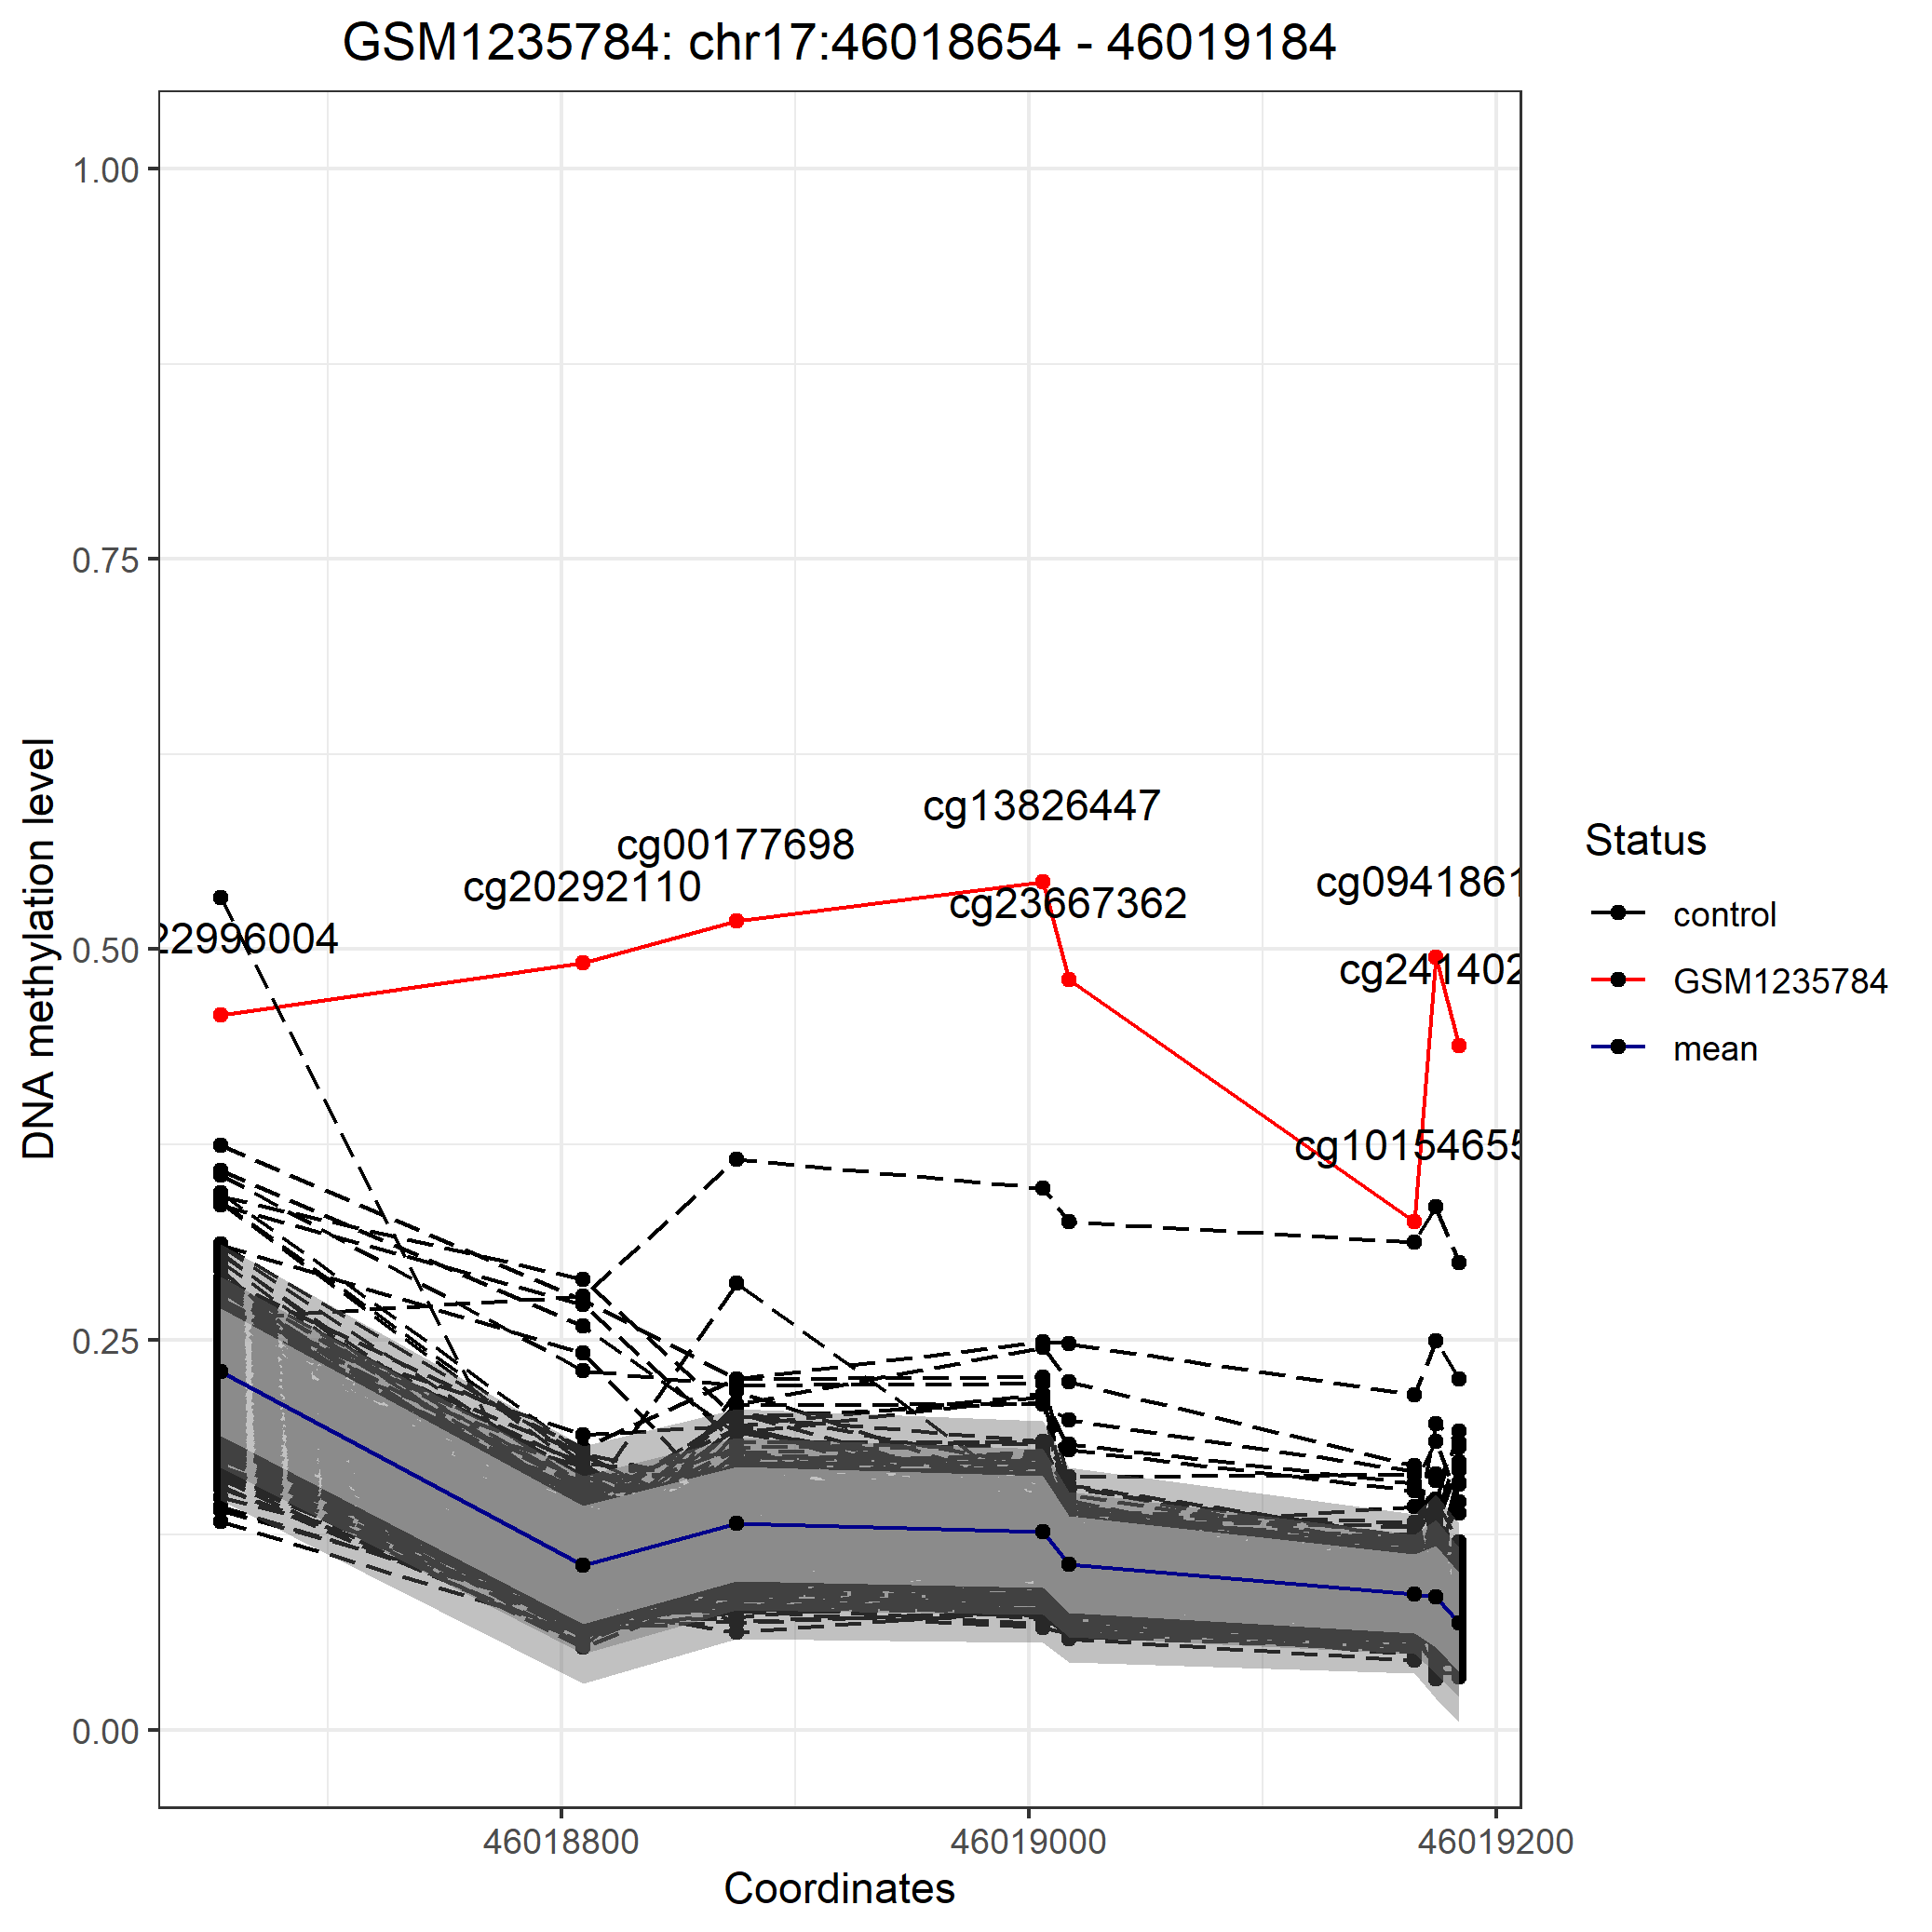
\includegraphics[width=28.82in]{C:/Users/nla94/Documents/GitHub/Supplementary-Material/Abarrategui_2021/vignette/fig/GSM1235784_chr17-46018654-46019184} 

}

\caption{GSE51032 samples in the region chr17:46018654-46019184}\label{fig:graph_GSM1235784}
\end{figure}

\begin{figure}[H]

{\centering 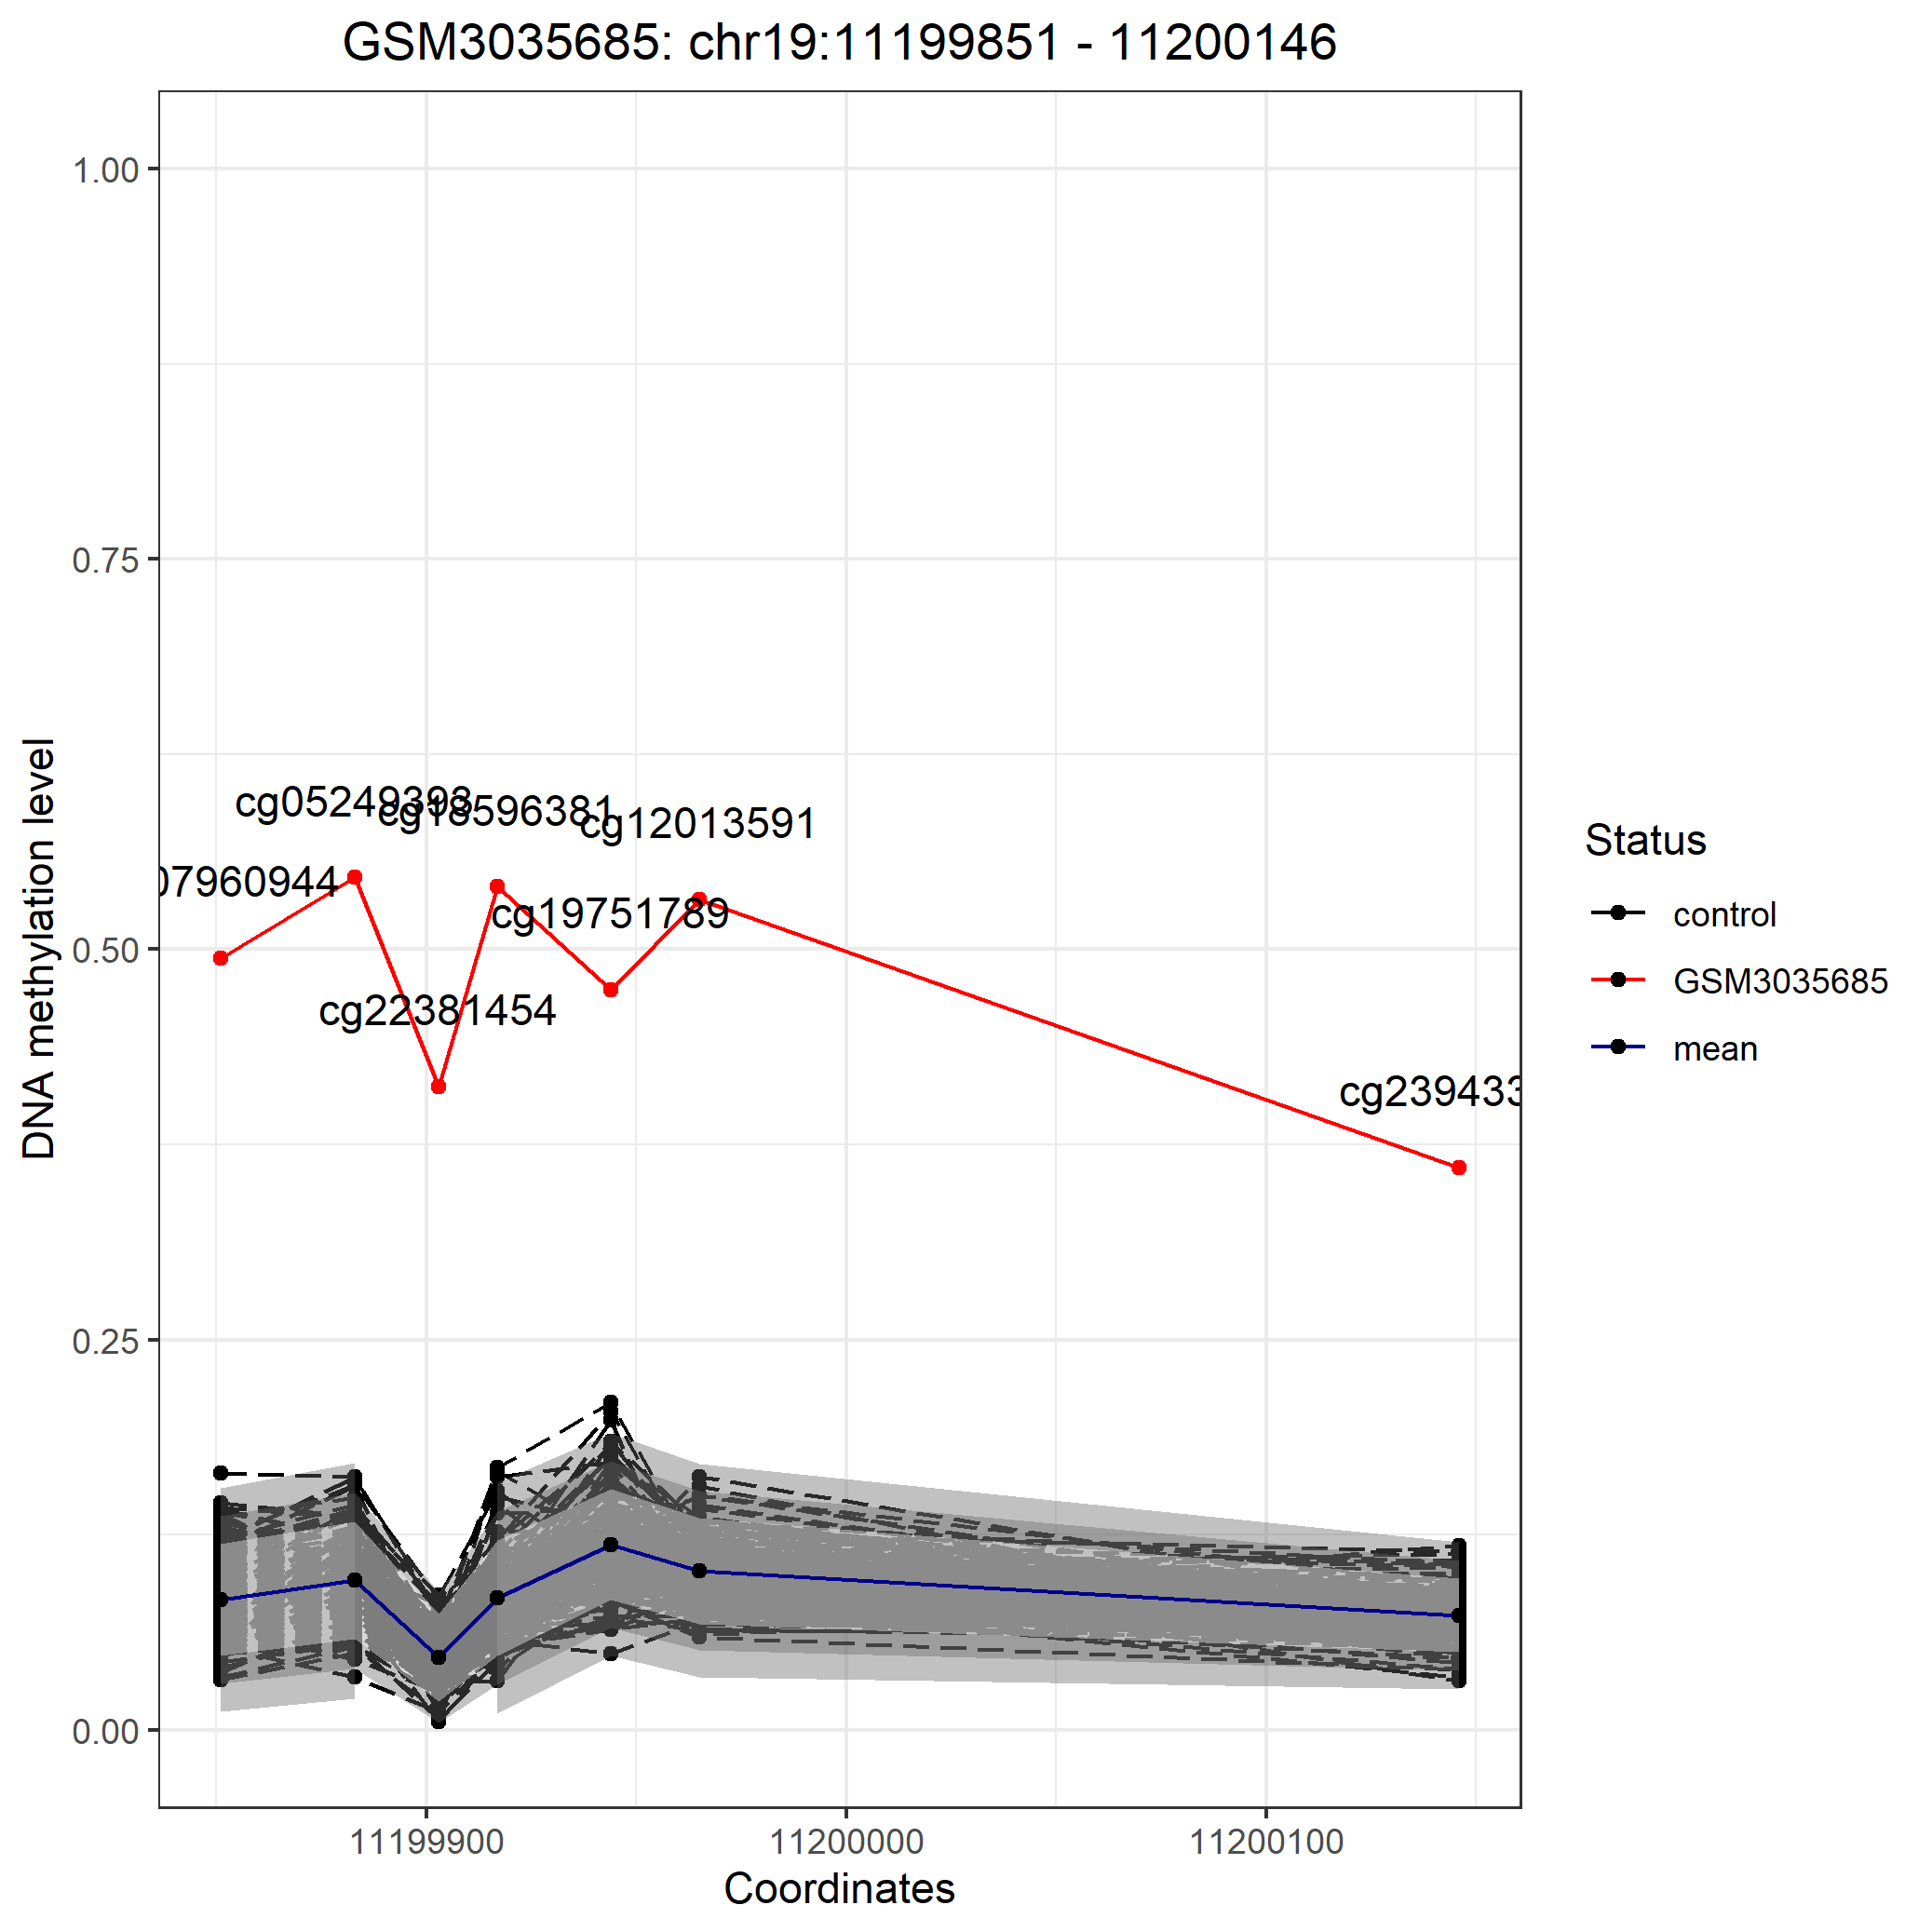
\includegraphics[width=28.82in]{C:/Users/nla94/Documents/GitHub/Supplementary-Material/Abarrategui_2021/vignette/fig/GSM3035685_chr19-11199851-11200146} 

}

\caption{GSE111629 samples in the region chr19:11199851-11200146}\label{fig:graph_GSM3035685}
\end{figure}

\begin{figure}[H]

{\centering 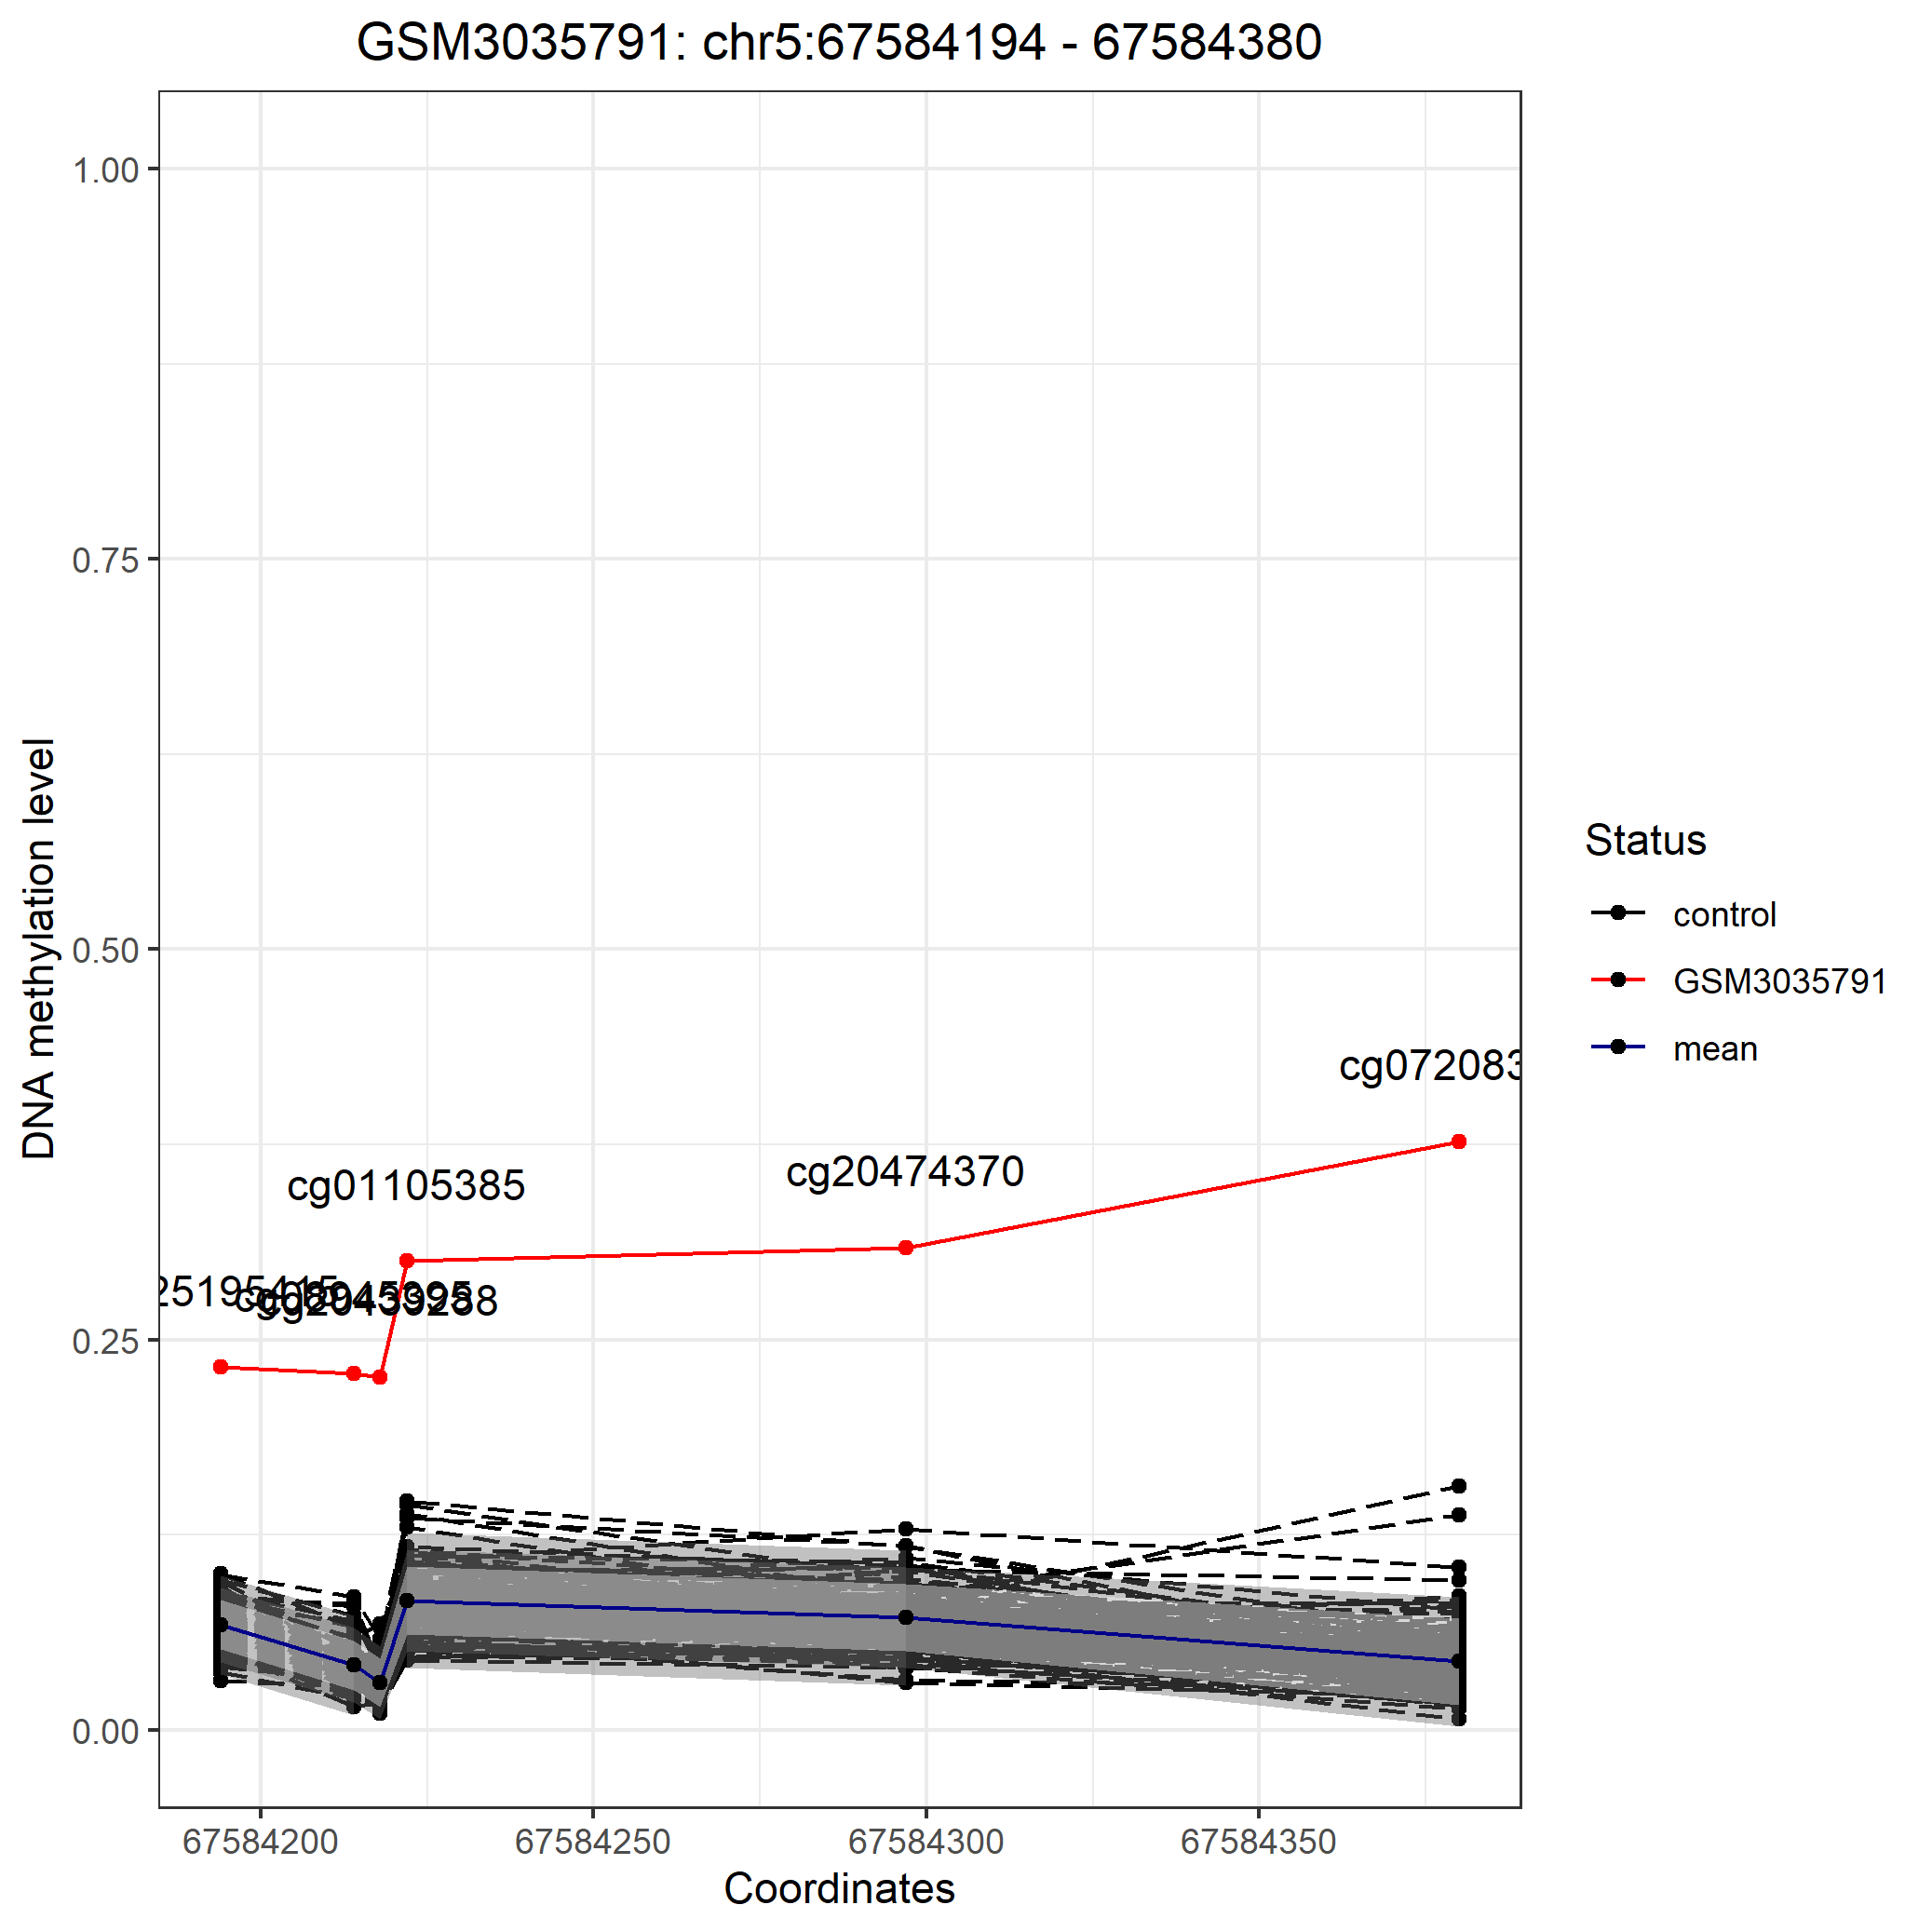
\includegraphics[width=28.82in]{C:/Users/nla94/Documents/GitHub/Supplementary-Material/Abarrategui_2021/vignette/fig/GSM3035791_chr5-67584194-67584380} 

}

\caption{GSE111629 samples in the region chr5:67584194-67584380}\label{fig:graph_GSM3035791}
\end{figure}

\begin{figure}[H]

{\centering 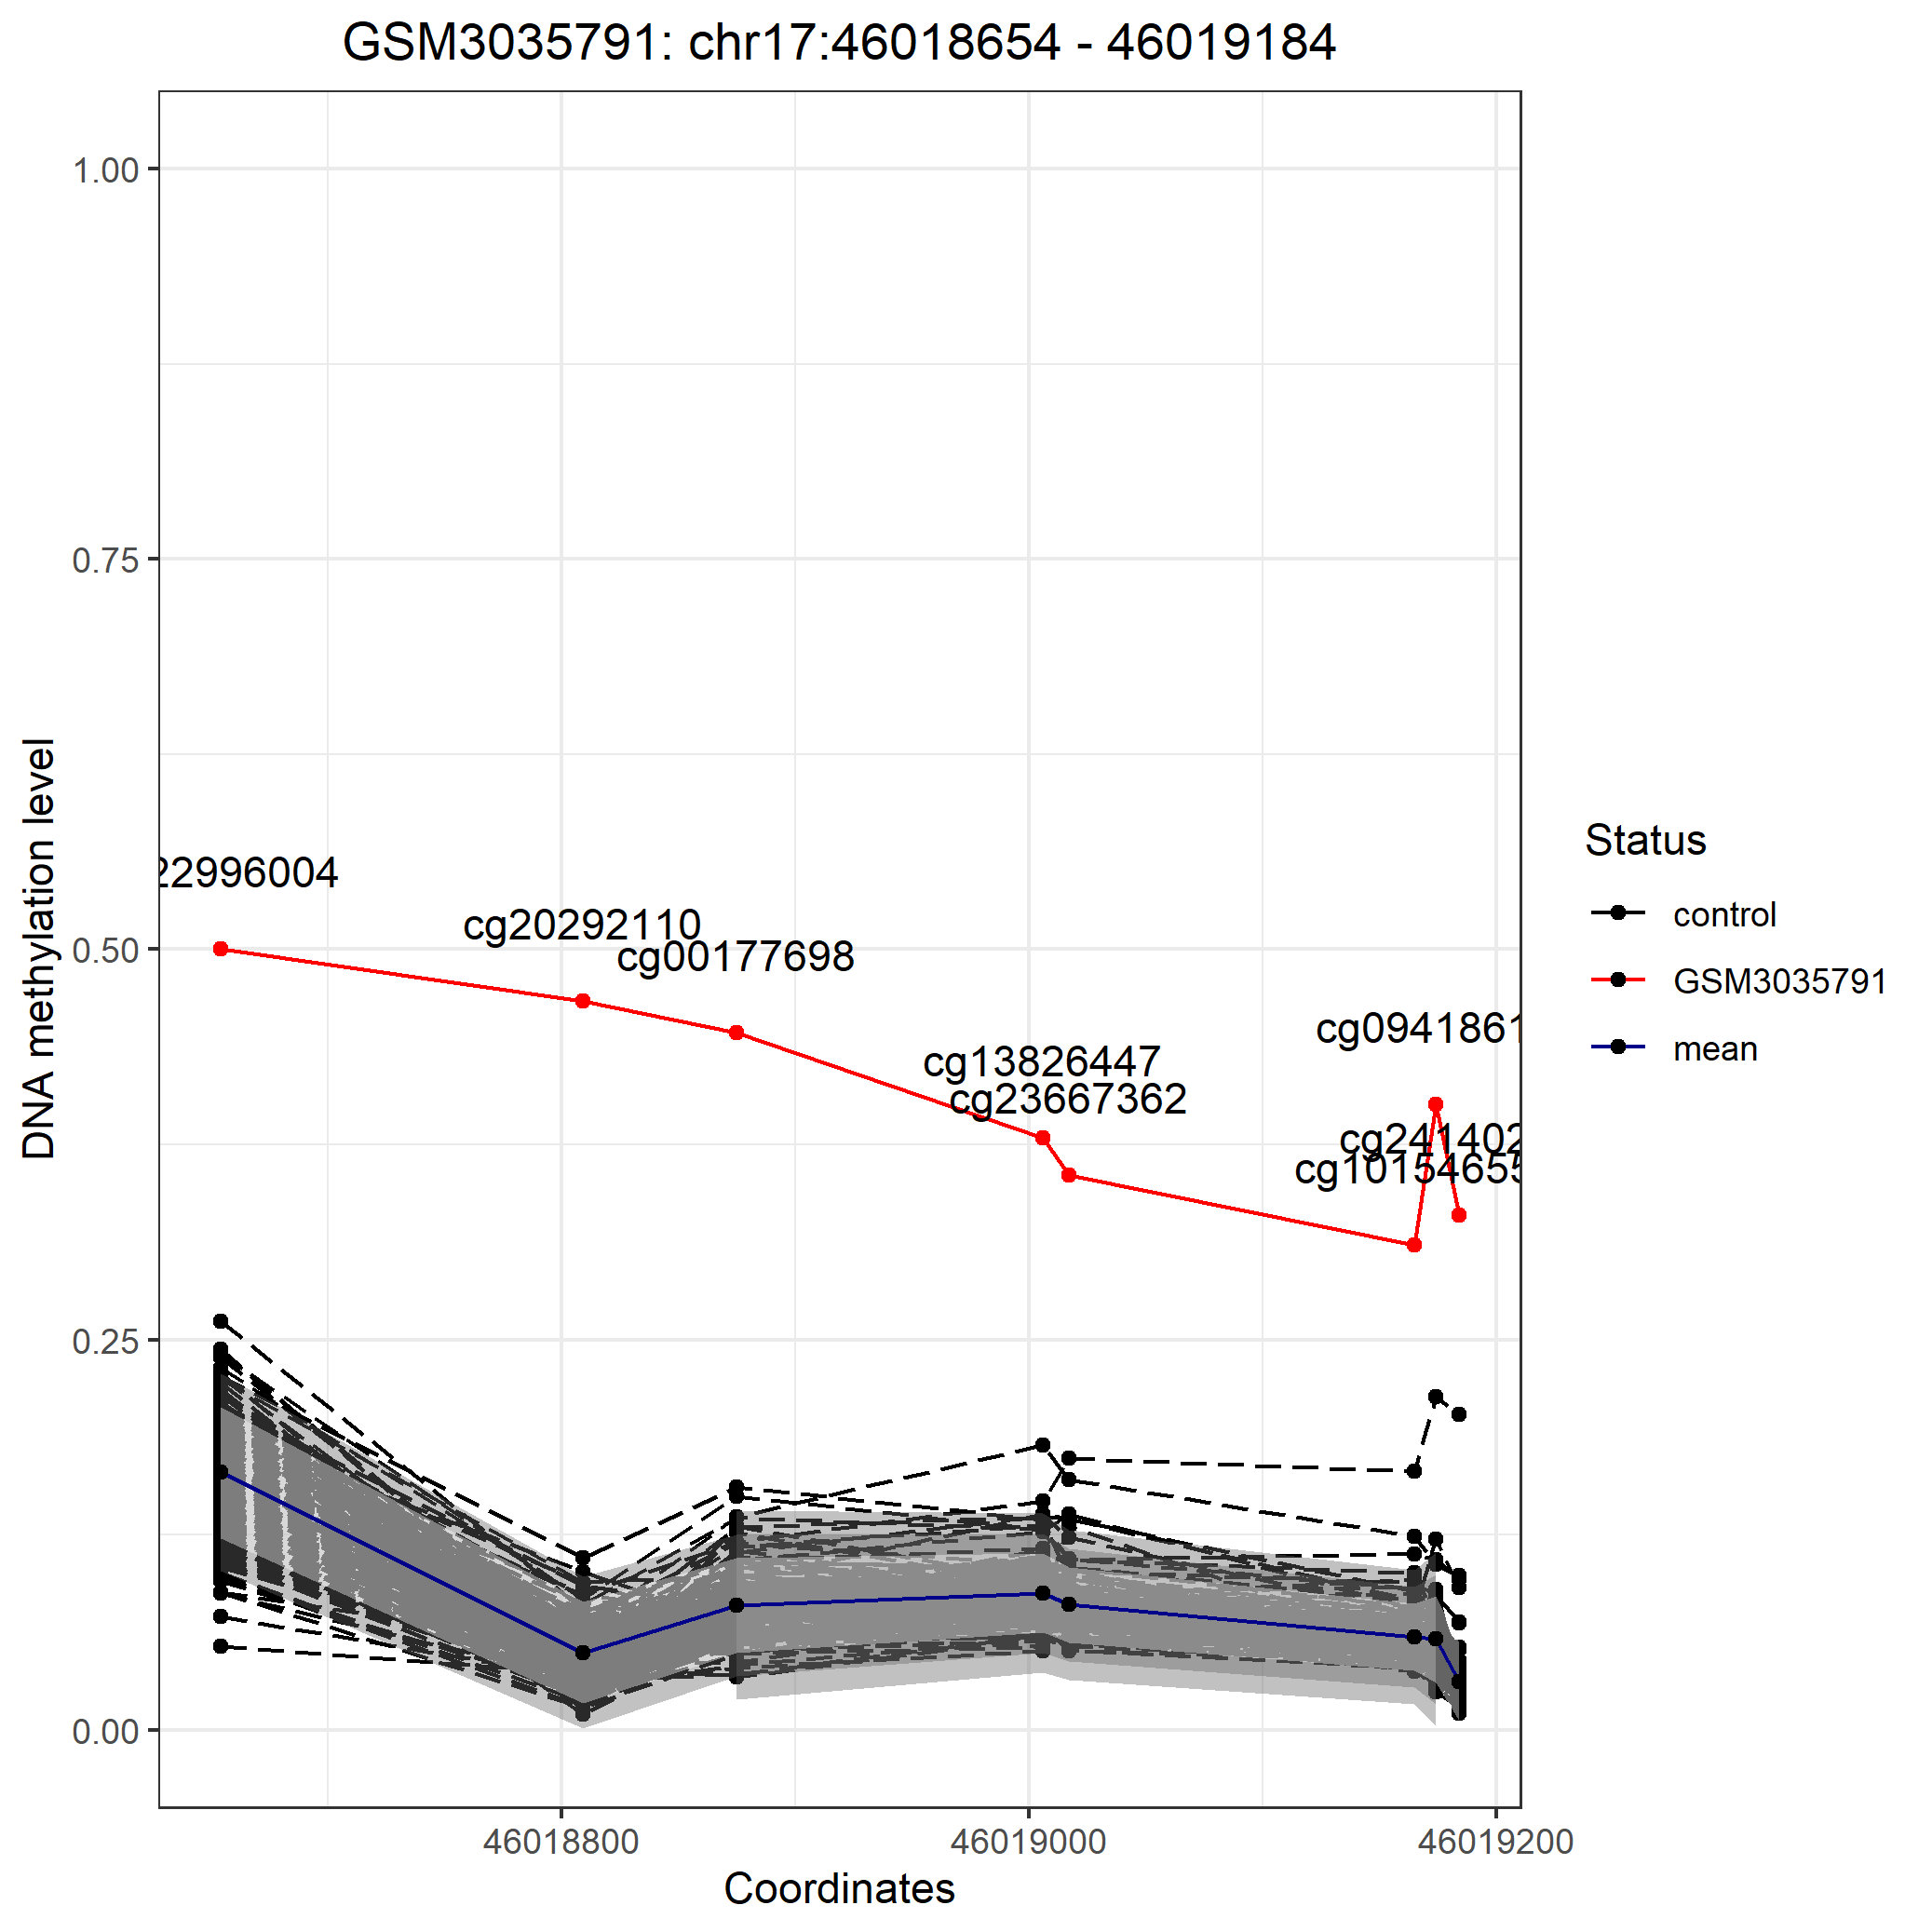
\includegraphics[width=28.82in]{C:/Users/nla94/Documents/GitHub/Supplementary-Material/Abarrategui_2021/vignette/fig/GSM3035791_chr17-46018654-46019184} 

}

\caption{GSE111629 samples in the region chr17:46018654-46019184}\label{fig:graph_GSM3035791.2}
\end{figure}

\begin{figure}[H]

{\centering 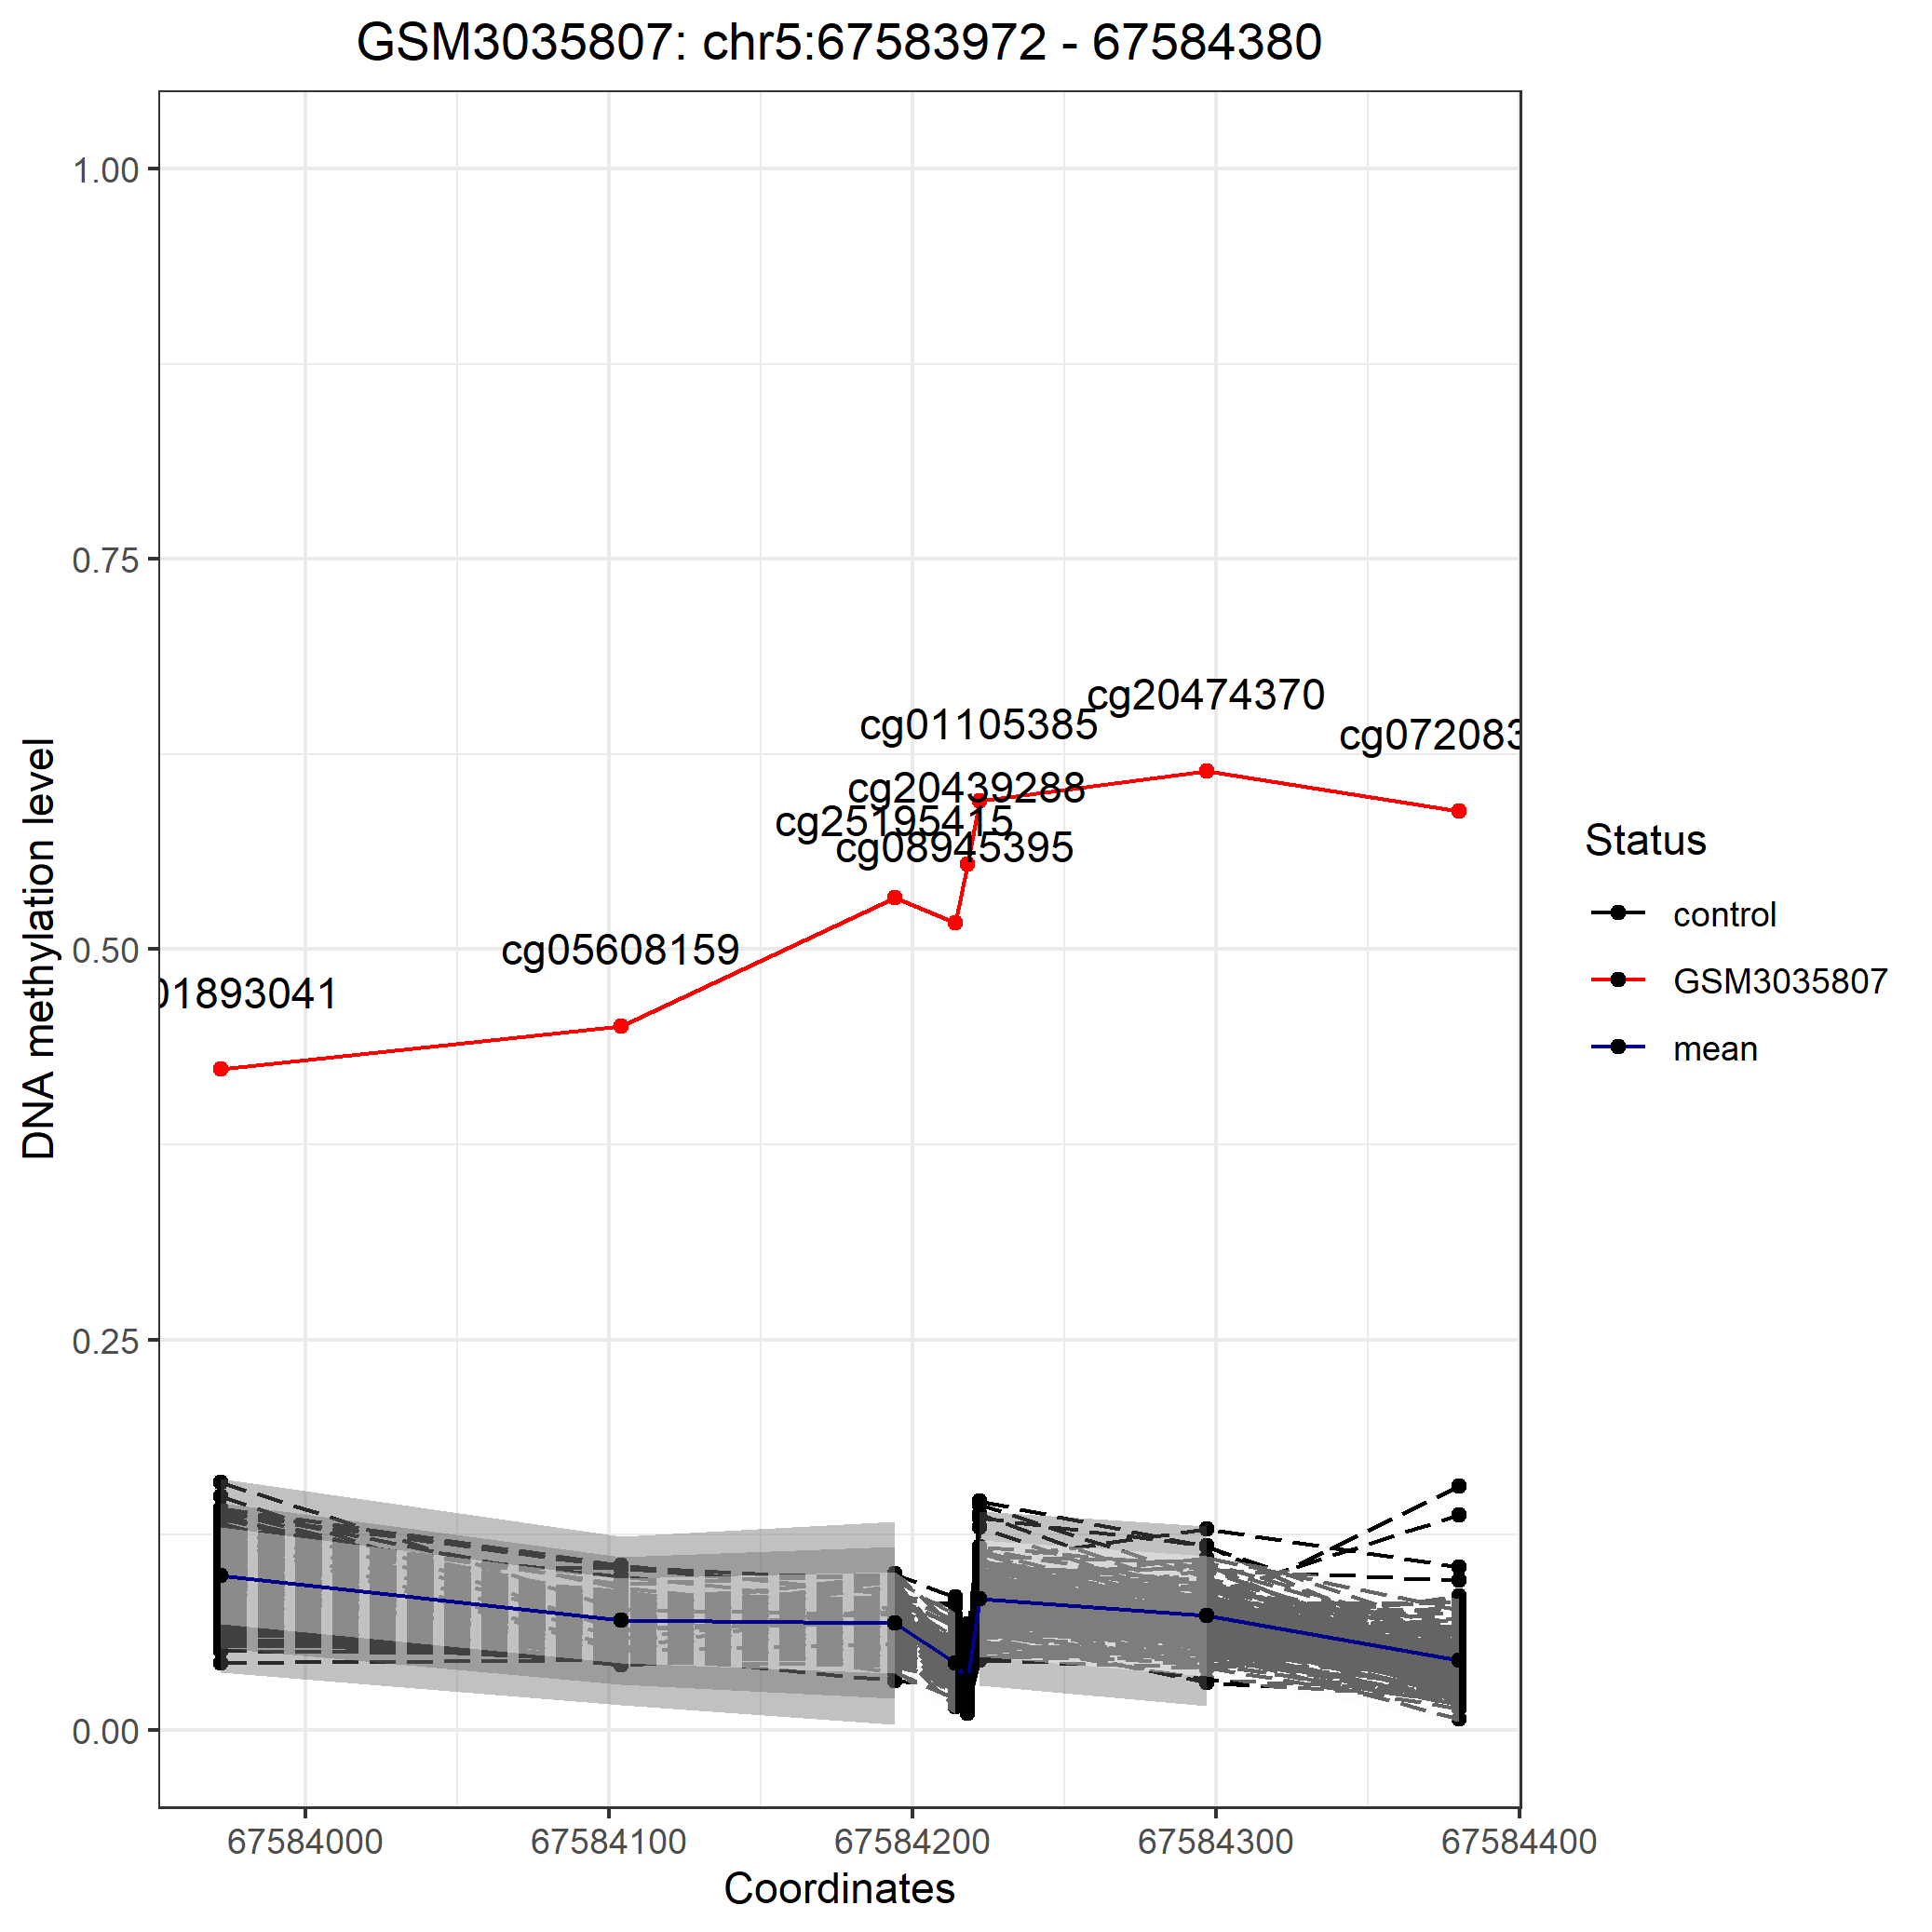
\includegraphics[width=28.82in]{C:/Users/nla94/Documents/GitHub/Supplementary-Material/Abarrategui_2021/vignette/fig/GSM3035807_chr5-67583972-67584380} 

}

\caption{GSE111629 samples in the region chr5:67583972-67584380}\label{fig:graph_GSM3035807}
\end{figure}

\begin{figure}[H]

{\centering 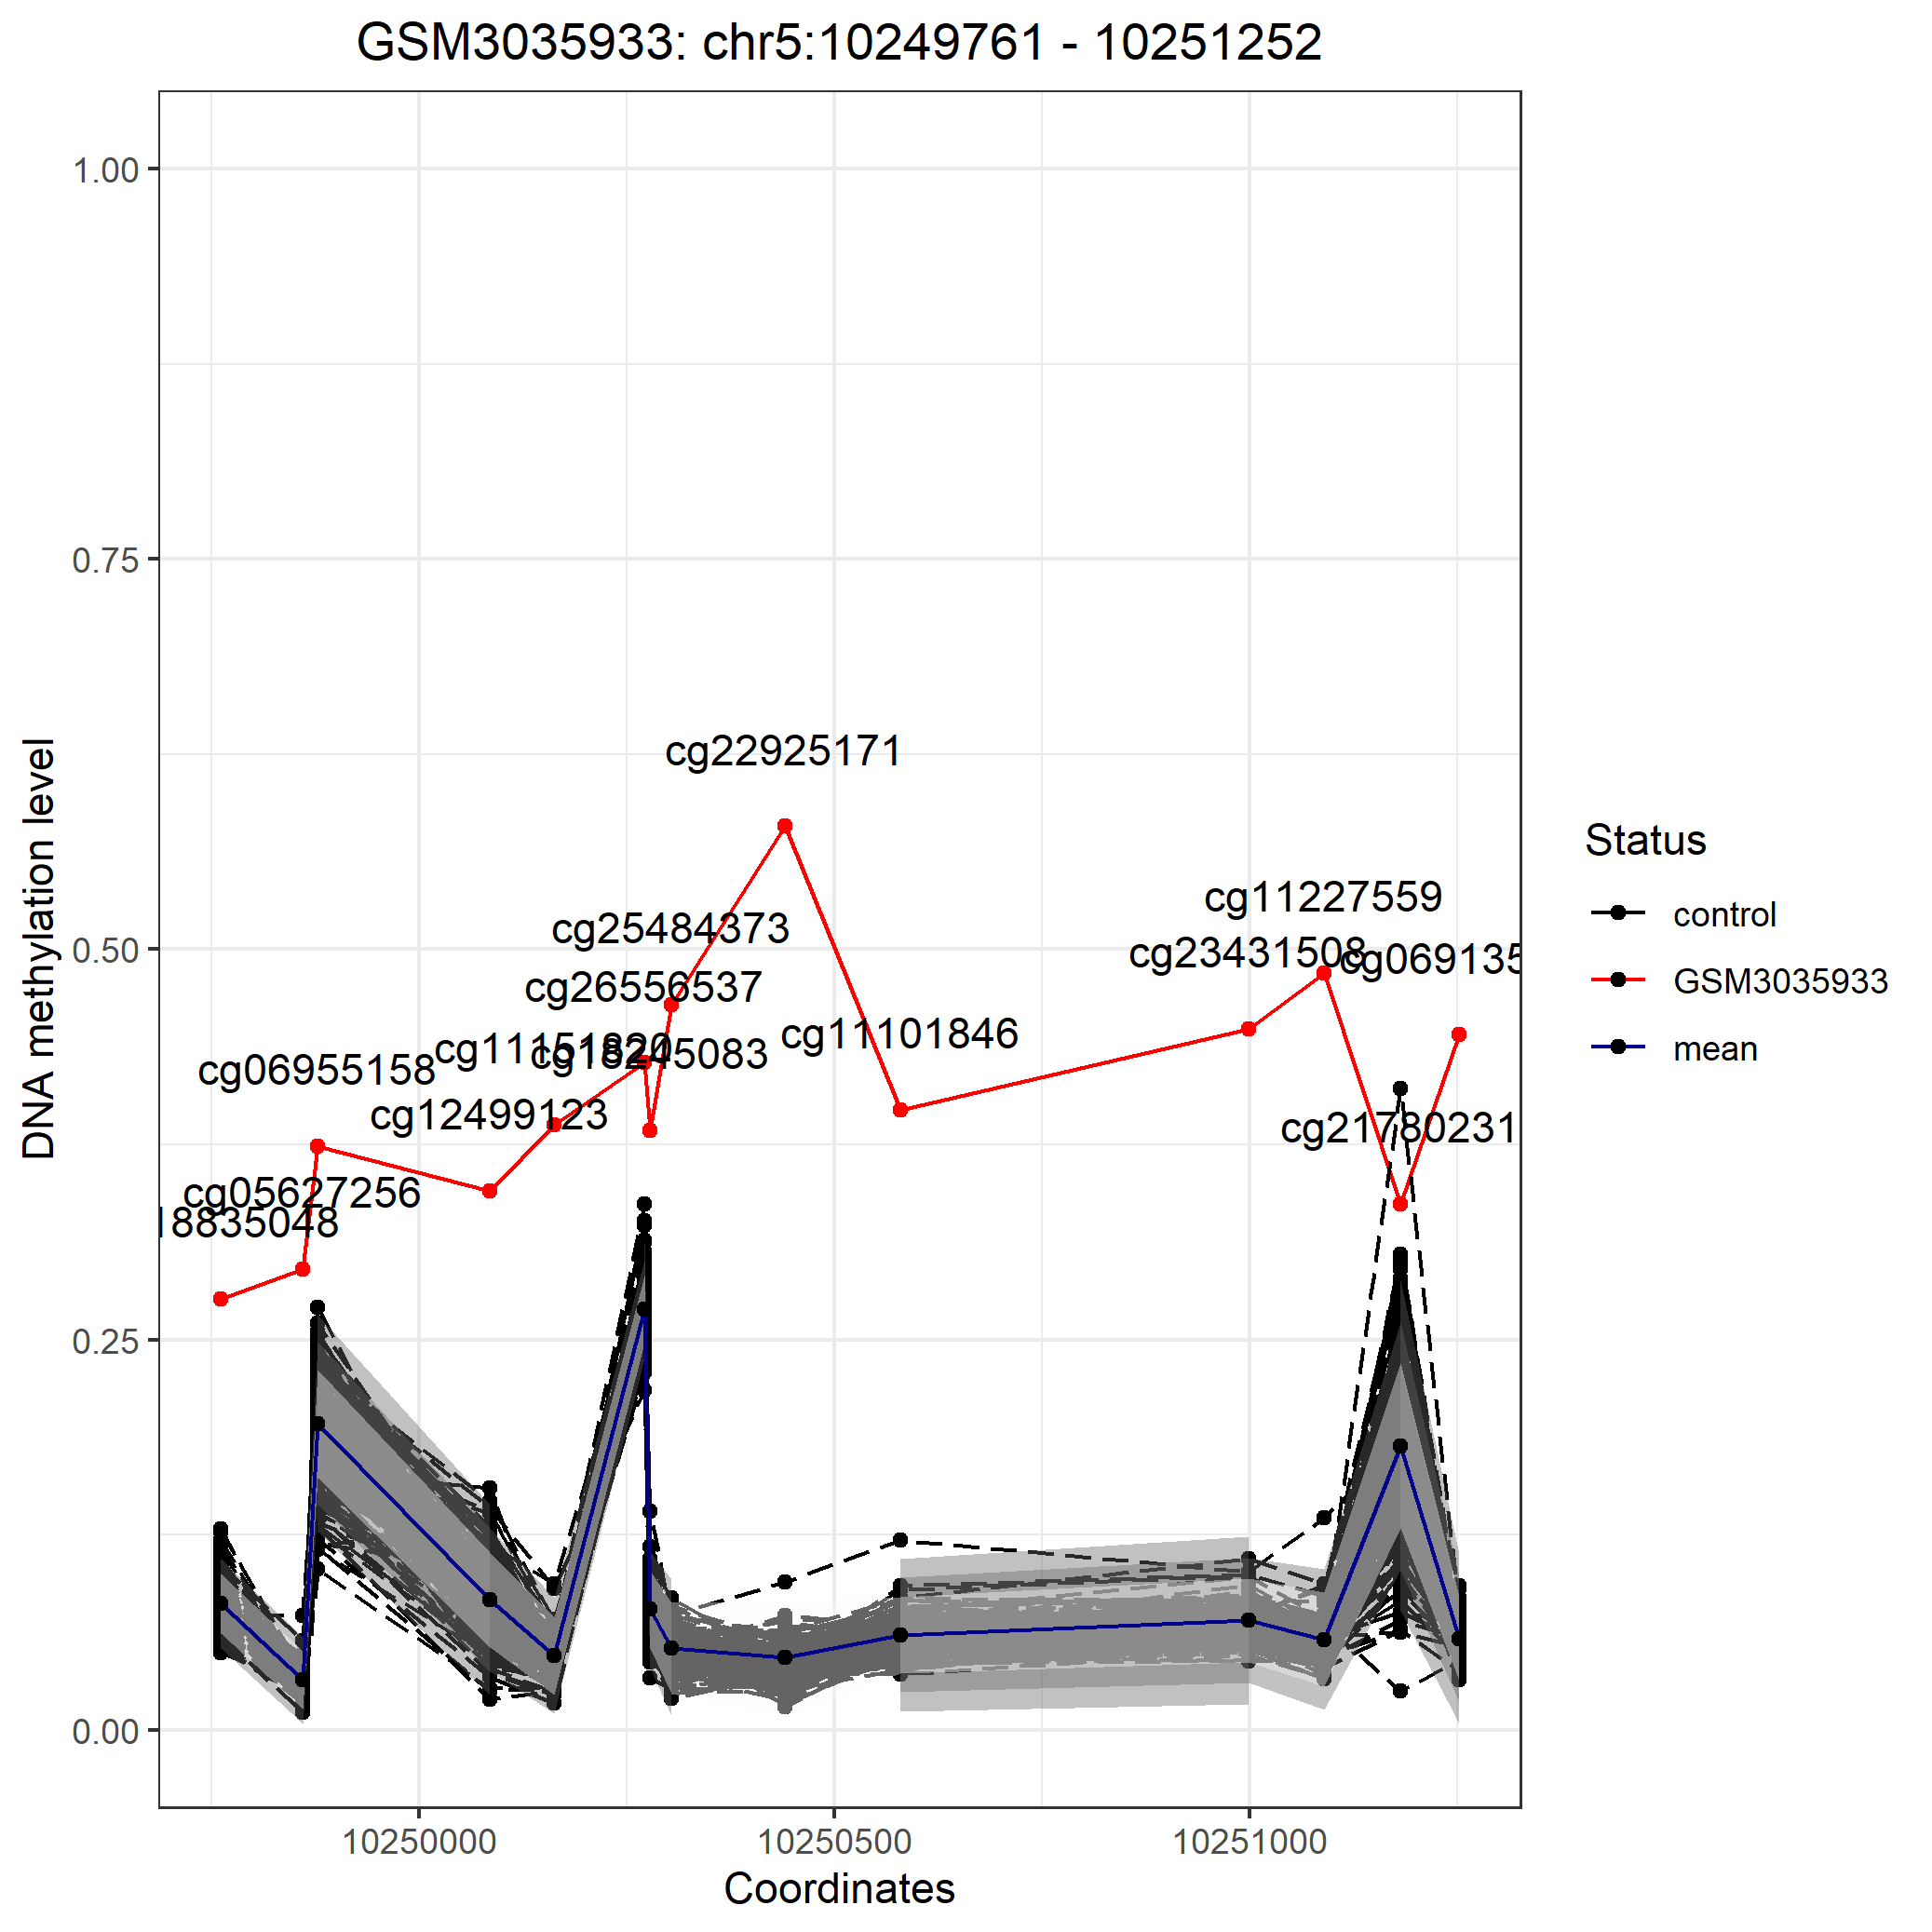
\includegraphics[width=28.82in]{C:/Users/nla94/Documents/GitHub/Supplementary-Material/Abarrategui_2021/vignette/fig/GSM3035933_chr5-10249761-10251252} 

}

\caption{GSE111629 samples in the region chr5:10249761-10251252}\label{fig:graph_GSM3035933}
\end{figure}

\hypertarget{results}{%
\subsection{Results}\label{results}}

We compare GSM1235784 case sample against randomly selected control
samples from GSE51032 and GSM3035933, GSM3035791, GSM3035807 and
GSM3035685 case samples against controls from GSE111629 specifying a
region of 20 kb and \(\ge\) 3 GpGs.

We obtained similar results in both cohorts. We observed that the
methods manova, mahalanobis distance and multivariate linear models
identified the validated epimutations with a TPR of \(>99\%\) even if
the control sample is small. However, the TPR in isolation forest
increases together with the number of control samples obtaining a TPR
\(\ge\) 75 with 50 control samples or more. The TPR in barbosa and beta
approaches for GSE51032 dataset is small (\(<50\%\)). Nonetheless, for
GSE111629 the TPR value increases considerably \(>99\%\). Regarding the
accuracy, all the statistical approaches detect the epivariants with
\(>80\%\) of closeness to the validated epimutations.

We detected possible epivariations outside the epimutations found by
(Garg et al. 2020) selecting control and case samples randomly. For the
analysis, we selected regions of 20 kb and \(\ge\) 3 GpGs. We compared
each case sample individually against control samples. We observed that
in both cohorts and for every approach the FPR value is very small
\(<0.01\%\).

\begin{table}
\centering
\begin{tabular}[t]{c|c|c|c}
\hline
method & TPR & accuracy & FPR\\
\hline
\multicolumn{4}{l}{\textbf{n20}}\\
\hline
\hspace{1em}manova & 98 & 99.6 & 0.00\\
\hline
\hspace{1em}mlm & 100 & 99.6 & \vphantom{8} 0.00\\
\hline
\hspace{1em}mahdistmcd & 100 & 99.6 & \vphantom{8} 0.00\\
\hline
\hspace{1em}isoforest & 28 & 99.6 & 0.00\\
\hline
\hspace{1em}barbosa & 100 & 94.4 & 0.25\\
\hline
\hspace{1em}beta & 99 & 89.0 & 0.25\\
\hline
\multicolumn{4}{l}{\textbf{n30}}\\
\hline
\hspace{1em}manova & 100 & 99.6 & \vphantom{7} 0.00\\
\hline
\hspace{1em}mlm & 100 & 99.6 & \vphantom{7} 0.00\\
\hline
\hspace{1em}mahdistmcd & 100 & 99.6 & \vphantom{7} 0.00\\
\hline
\hspace{1em}isoforest & 63 & 99.6 & 0.00\\
\hline
\hspace{1em}barbosa & 100 & 94.4 & 0.00\\
\hline
\hspace{1em}beta & 100 & 95.4 & 0.00\\
\hline
\multicolumn{4}{l}{\textbf{n40}}\\
\hline
\hspace{1em}manova & 100 & 99.6 & \vphantom{6} 0.00\\
\hline
\hspace{1em}mlm & 100 & 99.6 & \vphantom{6} 0.00\\
\hline
\hspace{1em}mahdistmcd & 100 & 99.6 & \vphantom{6} 0.00\\
\hline
\hspace{1em}isoforest & 65 & 99.6 & 0.00\\
\hline
\hspace{1em}barbosa & 100 & 92.4 & 0.00\\
\hline
\hspace{1em}beta & 100 & 92.6 & \vphantom{1} 0.00\\
\hline
\multicolumn{4}{l}{\textbf{n50}}\\
\hline
\hspace{1em}manova & 100 & 99.6 & \vphantom{5} 0.00\\
\hline
\hspace{1em}mlm & 100 & 99.6 & \vphantom{5} 0.00\\
\hline
\hspace{1em}mahdistmcd & 100 & 99.6 & \vphantom{5} 0.00\\
\hline
\hspace{1em}isoforest & 83 & 99.6 & 0.00\\
\hline
\hspace{1em}barbosa & 100 & 88.0 & 0.00\\
\hline
\hspace{1em}beta & 100 & 93.8 & 0.00\\
\hline
\multicolumn{4}{l}{\textbf{n60}}\\
\hline
\hspace{1em}manova & 100 & 99.6 & \vphantom{4} 0.00\\
\hline
\hspace{1em}mlm & 100 & 99.6 & \vphantom{4} 0.00\\
\hline
\hspace{1em}mahdistmcd & 100 & 99.6 & \vphantom{4} 0.00\\
\hline
\hspace{1em}isoforest & 88 & 99.6 & 0.00\\
\hline
\hspace{1em}barbosa & 100 & 89.2 & 0.00\\
\hline
\hspace{1em}beta & 100 & 92.6 & 0.00\\
\hline
\multicolumn{4}{l}{\textbf{n70}}\\
\hline
\hspace{1em}manova & 100 & 99.6 & \vphantom{3} 0.00\\
\hline
\hspace{1em}mlm & 100 & 99.6 & \vphantom{3} 0.00\\
\hline
\hspace{1em}mahdistmcd & 100 & 99.6 & \vphantom{3} 0.00\\
\hline
\hspace{1em}isoforest & 94 & 99.6 & 0.00\\
\hline
\hspace{1em}barbosa & 100 & 90.0 & 0.00\\
\hline
\hspace{1em}beta & 100 & 93.2 & 0.00\\
\hline
\multicolumn{4}{l}{\textbf{n80}}\\
\hline
\hspace{1em}manova & 100 & 99.6 & \vphantom{2} 0.00\\
\hline
\hspace{1em}mlm & 100 & 99.6 & \vphantom{2} 0.00\\
\hline
\hspace{1em}mahdistmcd & 100 & 99.6 & \vphantom{2} 0.00\\
\hline
\hspace{1em}isoforest & 97 & 99.6 & 0.00\\
\hline
\hspace{1em}barbosa & 100 & 86.0 & 0.00\\
\hline
\hspace{1em}beta & 100 & 92.9 & \vphantom{1} 0.00\\
\hline
\multicolumn{4}{l}{\textbf{n90}}\\
\hline
\hspace{1em}manova & 100 & 99.6 & \vphantom{1} 0.00\\
\hline
\hspace{1em}mlm & 100 & 99.6 & \vphantom{1} 0.00\\
\hline
\hspace{1em}mahdistmcd & 100 & 99.6 & \vphantom{1} 0.00\\
\hline
\hspace{1em}isoforest & 98 & 99.6 & 0.00\\
\hline
\hspace{1em}barbosa & 100 & 81.3 & \vphantom{1} 0.00\\
\hline
\hspace{1em}beta & 100 & 92.9 & 0.00\\
\hline
\multicolumn{4}{l}{\textbf{n100}}\\
\hline
\hspace{1em}manova & 100 & 99.6 & 0.00\\
\hline
\hspace{1em}mlm & 100 & 99.6 & 0.00\\
\hline
\hspace{1em}mahdistmcd & 100 & 99.6 & 0.00\\
\hline
\hspace{1em}isoforest & 99 & 99.6 & 0.00\\
\hline
\hspace{1em}barbosa & 100 & 81.3 & 0.00\\
\hline
\hspace{1em}beta & 100 & 90.3 & 0.00\\
\hline
\end{tabular}
\end{table}

\begin{figure}[H]

{\centering 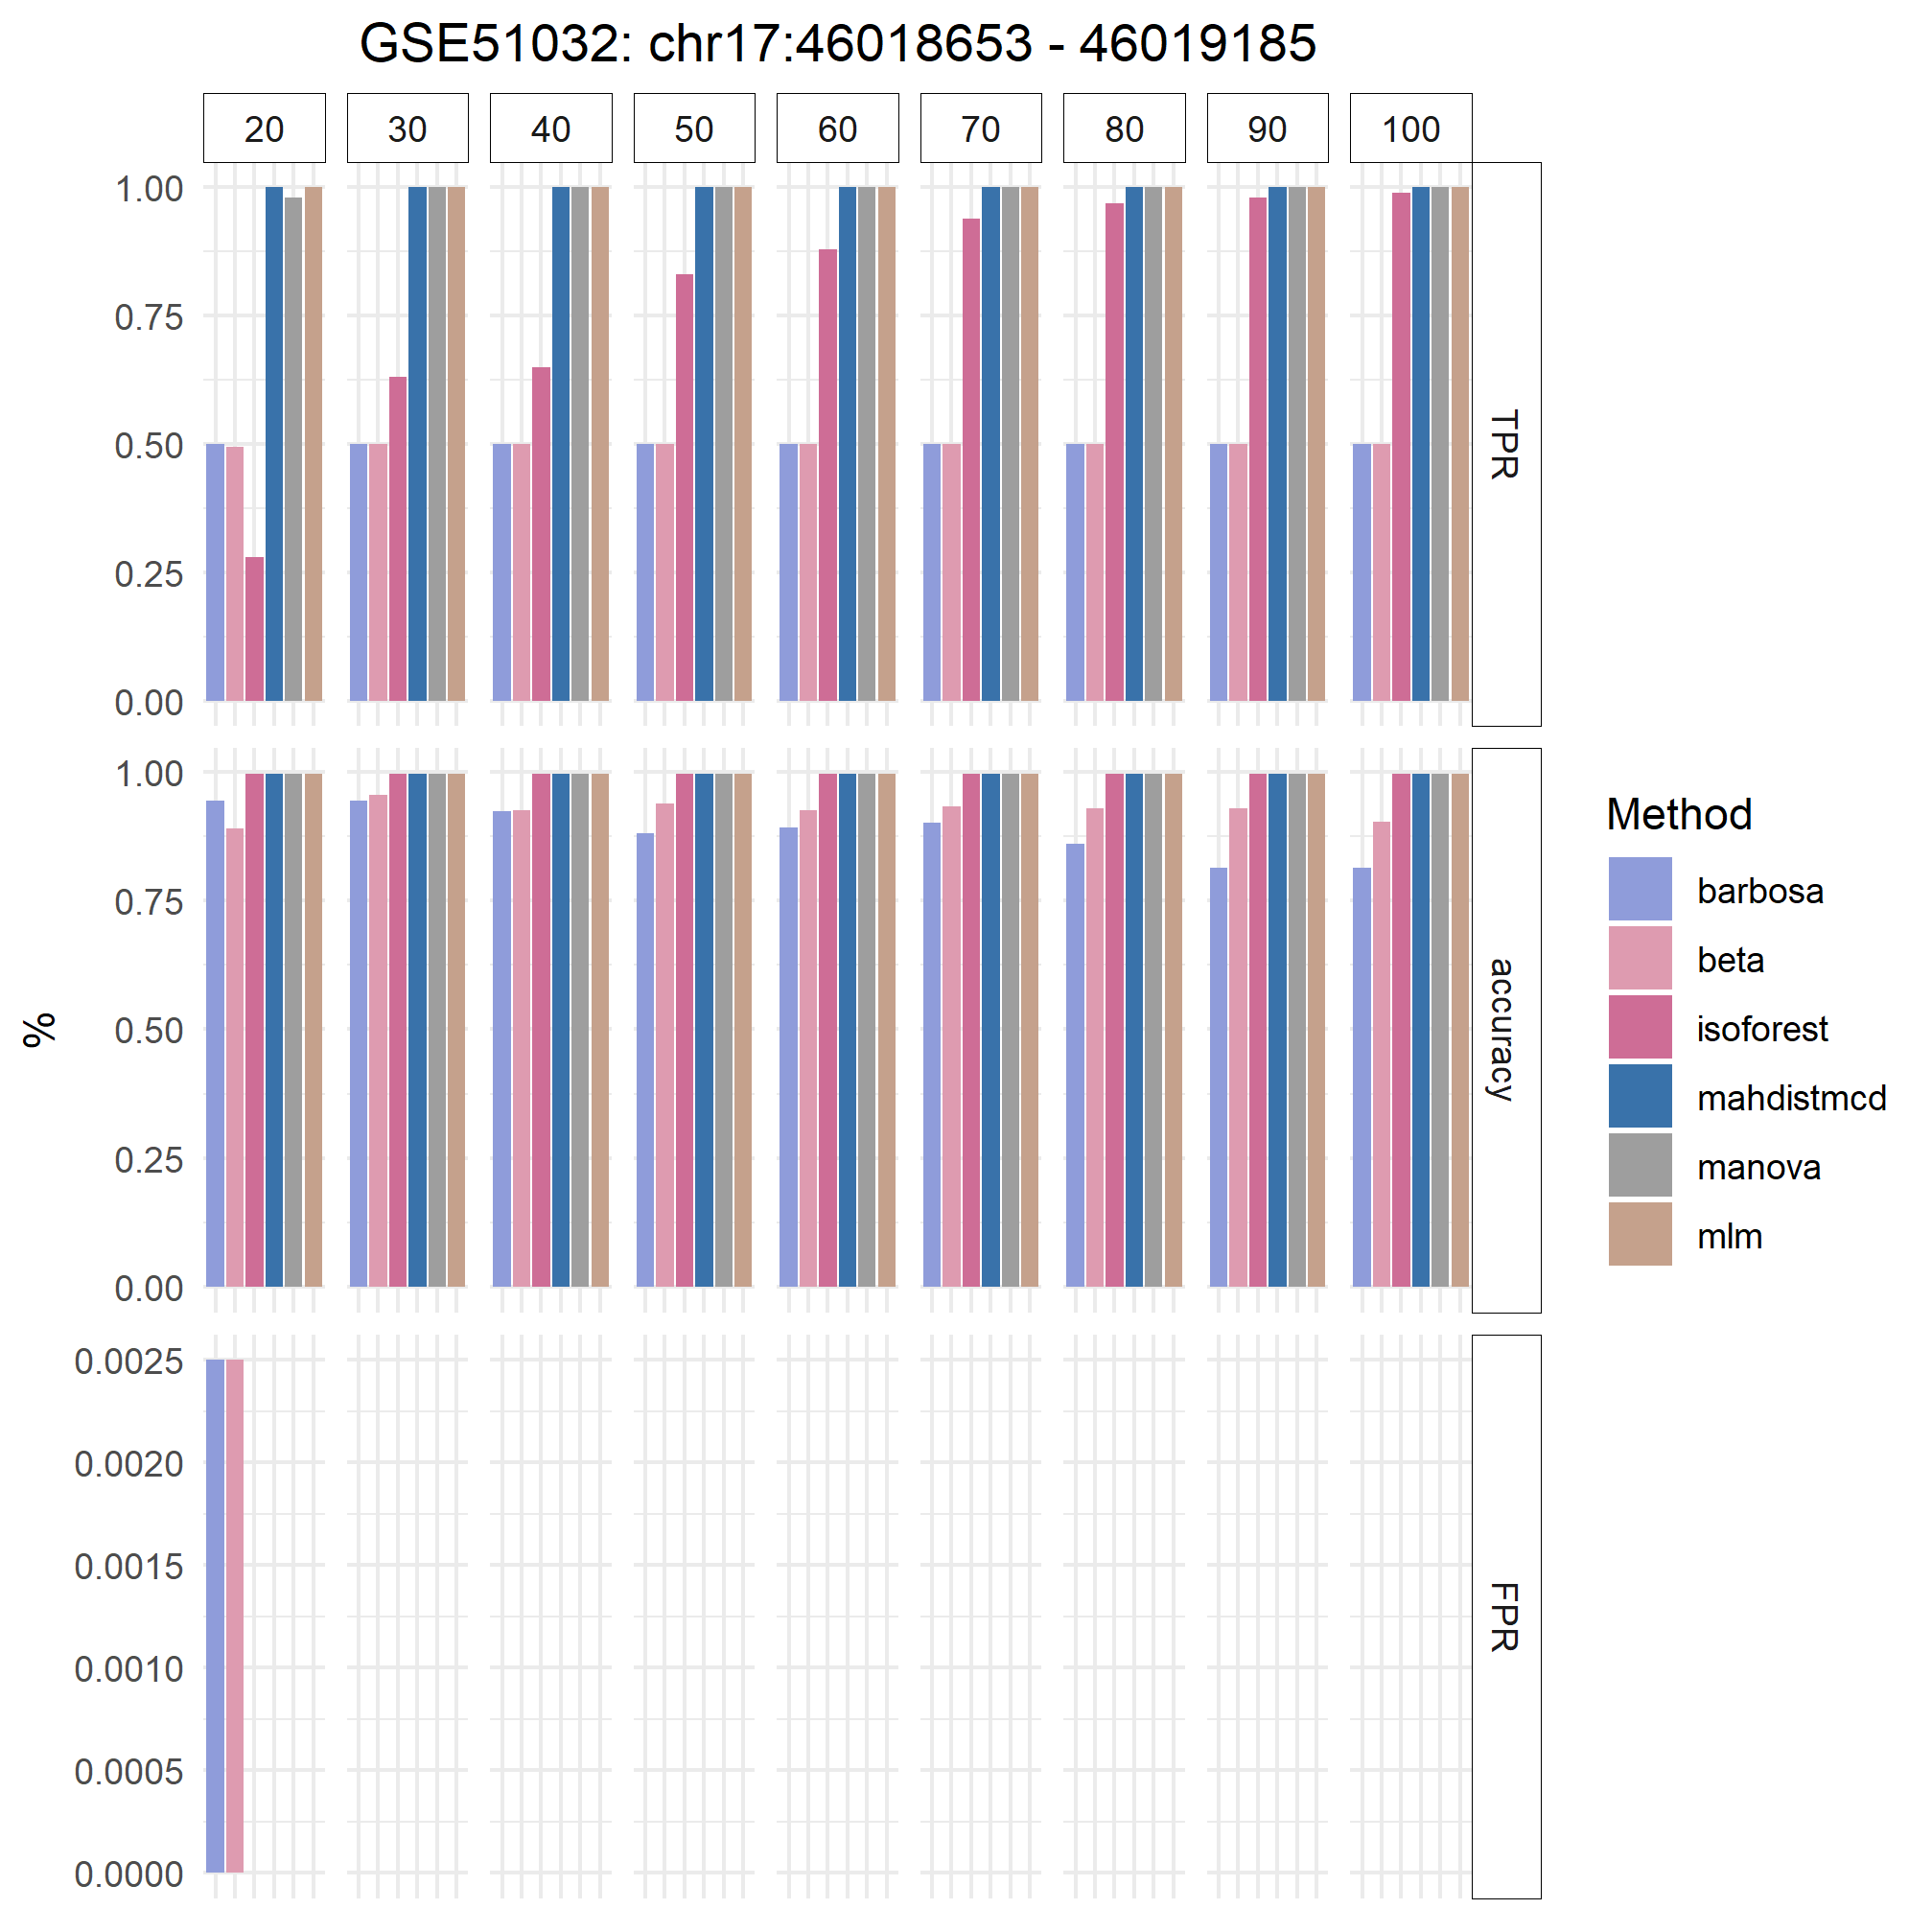
\includegraphics[width=27.99in]{C:/Users/nla94/Documents/GitHub/Supplementary-Material/Abarrategui_2021/result_files/4-Graph/GSE51032_chr17_46018653_46019185} 

}

\caption{epimutations performance for GSE51032 cohort detecting the epivariation located in chr5:10249760-10251253}\label{fig:graph_GSE51032}
\end{figure}

\begin{table}
\centering
\begin{tabular}[t]{c|c|c|c|c}
\hline
method & n & TPR & accuracy & FPR\\
\hline
\multicolumn{5}{l}{\textbf{n20}}\\
\hline
\hspace{1em}barbosa & 100 & 100.000 & 92.825 & 0.00\\
\hline
\hspace{1em}beta & 100 & 100.000 & 92.825 & 0.25\\
\hline
\hspace{1em}isoforest & 100 & 98.625 & 93.000 & 0.00\\
\hline
\hspace{1em}mahdistmcd & 100 & 100.000 & 92.825 & 0.00\\
\hline
\hspace{1em}manova & 100 & 100.000 & 92.825 & 0.00\\
\hline
\hspace{1em}mlm & 100 & 100.000 & 92.825 & 0.00\\
\hline
\multicolumn{5}{l}{\textbf{n30}}\\
\hline
\hspace{1em}barbosa & 20 & 100.000 & 92.825 & 0.00\\
\hline
\hspace{1em}beta & 20 & 87.500 & 92.800 & 0.00\\
\hline
\hspace{1em}isoforest & 20 & 11.500 & 86.800 & 0.00\\
\hline
\hspace{1em}mahdistmcd & 20 & 100.000 & 92.825 & 0.00\\
\hline
\hspace{1em}manova & 20 & 98.000 & 92.825 & 0.00\\
\hline
\hspace{1em}mlm & 20 & 100.000 & 92.850 & 0.00\\
\hline
\multicolumn{5}{l}{\textbf{n40}}\\
\hline
\hspace{1em}barbosa & 30 & 100.000 & 92.825 & 0.25\\
\hline
\hspace{1em}beta & 30 & 87.500 & 92.775 & 0.25\\
\hline
\hspace{1em}isoforest & 30 & 28.000 & 93.150 & 0.00\\
\hline
\hspace{1em}mahdistmcd & 30 & 100.000 & 92.825 & 0.00\\
\hline
\hspace{1em}manova & 30 & 100.000 & 92.825 & 0.00\\
\hline
\hspace{1em}mlm & 30 & 100.000 & 92.825 & 0.00\\
\hline
\multicolumn{5}{l}{\textbf{n50}}\\
\hline
\hspace{1em}barbosa & 40 & 100.000 & 92.825 & 0.00\\
\hline
\hspace{1em}beta & 40 & 87.500 & 92.800 & 0.00\\
\hline
\hspace{1em}isoforest & 40 & 46.375 & 93.950 & 0.00\\
\hline
\hspace{1em}mahdistmcd & 40 & 100.000 & 92.825 & 0.00\\
\hline
\hspace{1em}manova & 40 & 100.000 & 92.825 & 0.00\\
\hline
\hspace{1em}mlm & 40 & 100.000 & 92.825 & 0.00\\
\hline
\multicolumn{5}{l}{\textbf{n60}}\\
\hline
\hspace{1em}barbosa & 50 & 100.000 & 92.825 & 0.00\\
\hline
\hspace{1em}beta & 50 & 87.500 & 92.825 & 0.00\\
\hline
\hspace{1em}isoforest & 50 & 70.125 & 93.500 & 0.00\\
\hline
\hspace{1em}mahdistmcd & 50 & 100.000 & 92.825 & 0.00\\
\hline
\hspace{1em}manova & 50 & 100.000 & 92.825 & 0.00\\
\hline
\hspace{1em}mlm & 50 & 100.000 & 92.825 & 0.00\\
\hline
\multicolumn{5}{l}{\textbf{n70}}\\
\hline
\hspace{1em}barbosa & 60 & 100.000 & 92.825 & 0.00\\
\hline
\hspace{1em}beta & 60 & 100.000 & 92.825 & 0.00\\
\hline
\hspace{1em}isoforest & 60 & 78.750 & 93.500 & 0.00\\
\hline
\hspace{1em}mahdistmcd & 60 & 100.000 & 92.825 & 0.00\\
\hline
\hspace{1em}manova & 60 & 100.000 & 92.825 & 0.00\\
\hline
\hspace{1em}mlm & 60 & 100.000 & 92.825 & 0.00\\
\hline
\multicolumn{5}{l}{\textbf{n80}}\\
\hline
\hspace{1em}barbosa & 70 & 100.000 & 92.825 & 0.25\\
\hline
\hspace{1em}beta & 70 & 100.000 & 92.825 & 0.00\\
\hline
\hspace{1em}isoforest & 70 & 90.125 & 93.575 & 0.00\\
\hline
\hspace{1em}mahdistmcd & 70 & 100.000 & 92.825 & 0.00\\
\hline
\hspace{1em}manova & 70 & 100.000 & 92.825 & 0.00\\
\hline
\hspace{1em}mlm & 70 & 100.000 & 92.825 & 0.00\\
\hline
\multicolumn{5}{l}{\textbf{n90}}\\
\hline
\hspace{1em}barbosa & 80 & 100.000 & 92.825 & 0.00\\
\hline
\hspace{1em}beta & 80 & 100.000 & 92.825 & 0.00\\
\hline
\hspace{1em}isoforest & 80 & 96.375 & 93.075 & 0.00\\
\hline
\hspace{1em}mahdistmcd & 80 & 100.000 & 92.825 & 0.00\\
\hline
\hspace{1em}manova & 80 & 100.000 & 92.825 & 0.00\\
\hline
\hspace{1em}mlm & 80 & 100.000 & 92.825 & 0.00\\
\hline
\multicolumn{5}{l}{\textbf{n100}}\\
\hline
\hspace{1em}barbosa & 90 & 100.000 & 92.825 & 0.00\\
\hline
\hspace{1em}beta & 90 & 100.000 & 92.825 & 0.25\\
\hline
\hspace{1em}isoforest & 90 & 97.125 & 93.000 & 0.00\\
\hline
\hspace{1em}mahdistmcd & 90 & 100.000 & 92.825 & 0.00\\
\hline
\hspace{1em}manova & 90 & 100.000 & 92.825 & 0.00\\
\hline
\hspace{1em}mlm & 90 & 100.000 & 92.825 & 0.00\\
\hline
\end{tabular}
\end{table}

\begin{figure}[H]

{\centering 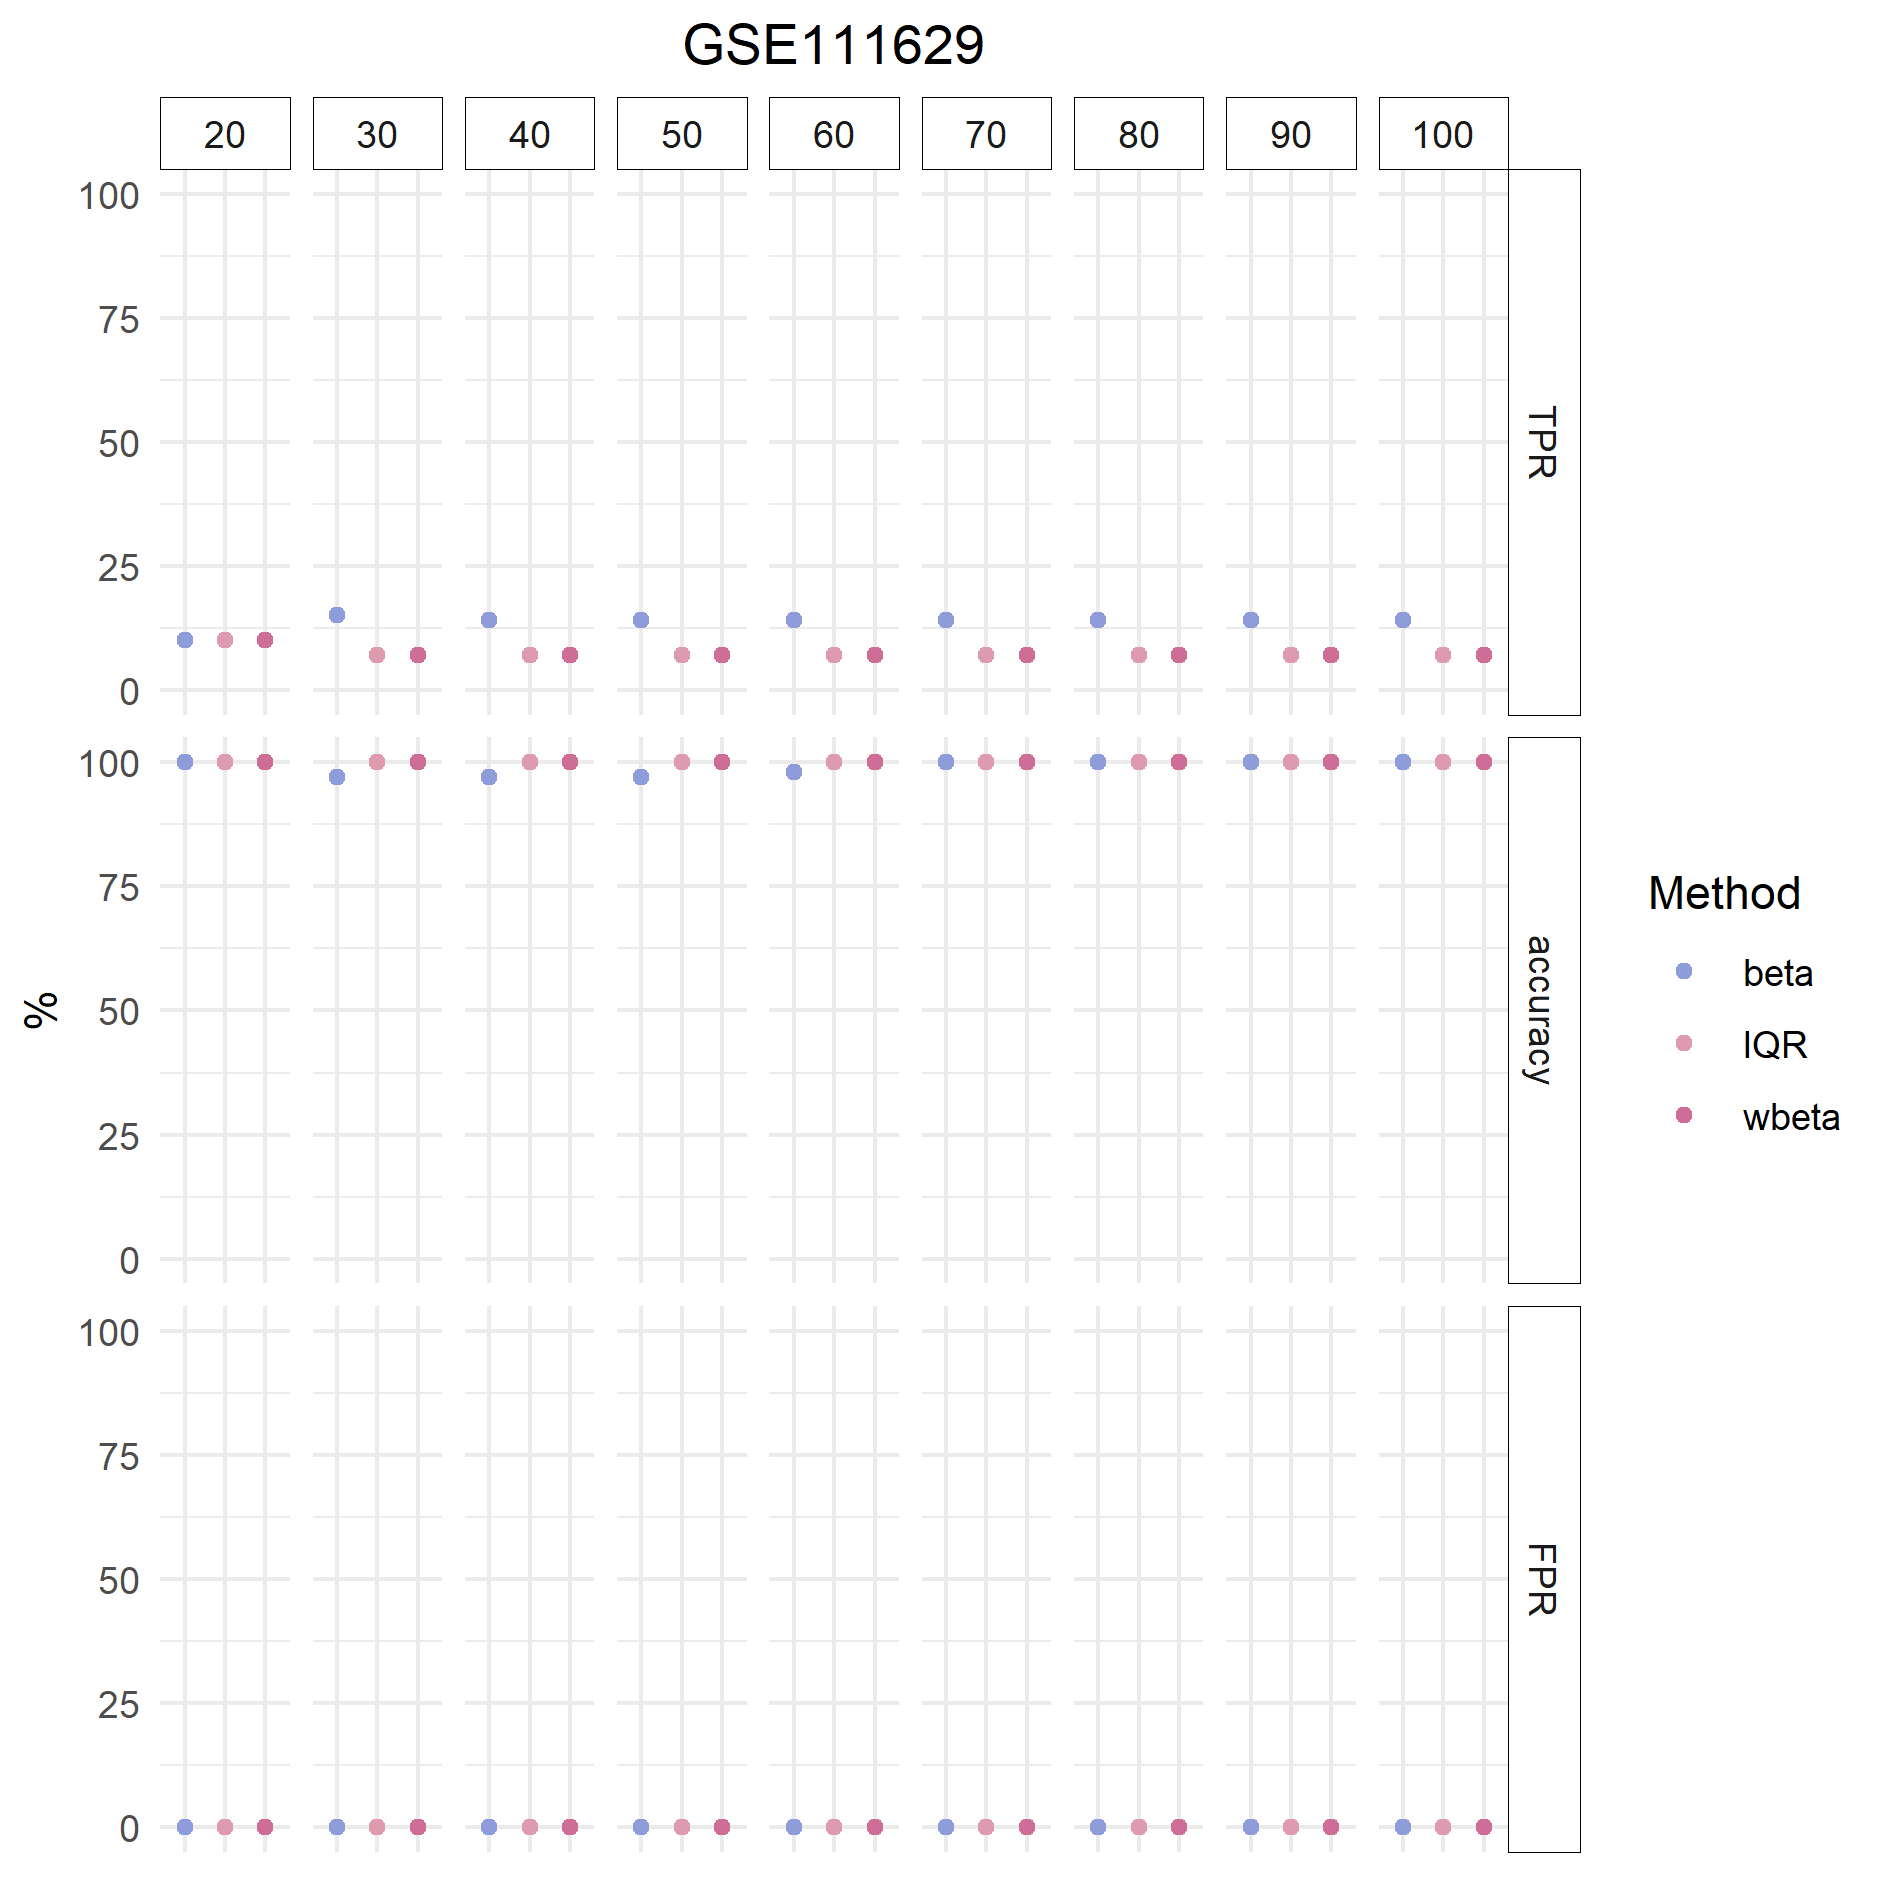
\includegraphics[width=27.99in]{C:/Users/nla94/Documents/GitHub/Supplementary-Material/Abarrategui_2021/result_files/4-Graph/GSE111629_chr5_10249760_10251253} 

}

\caption{epimutations performance using GSE111629 cohort to detect the epivariation located in chr5:10249760-10251253}\label{fig:graph_GSE111629_1}
\end{figure}

\begin{figure}

{\centering 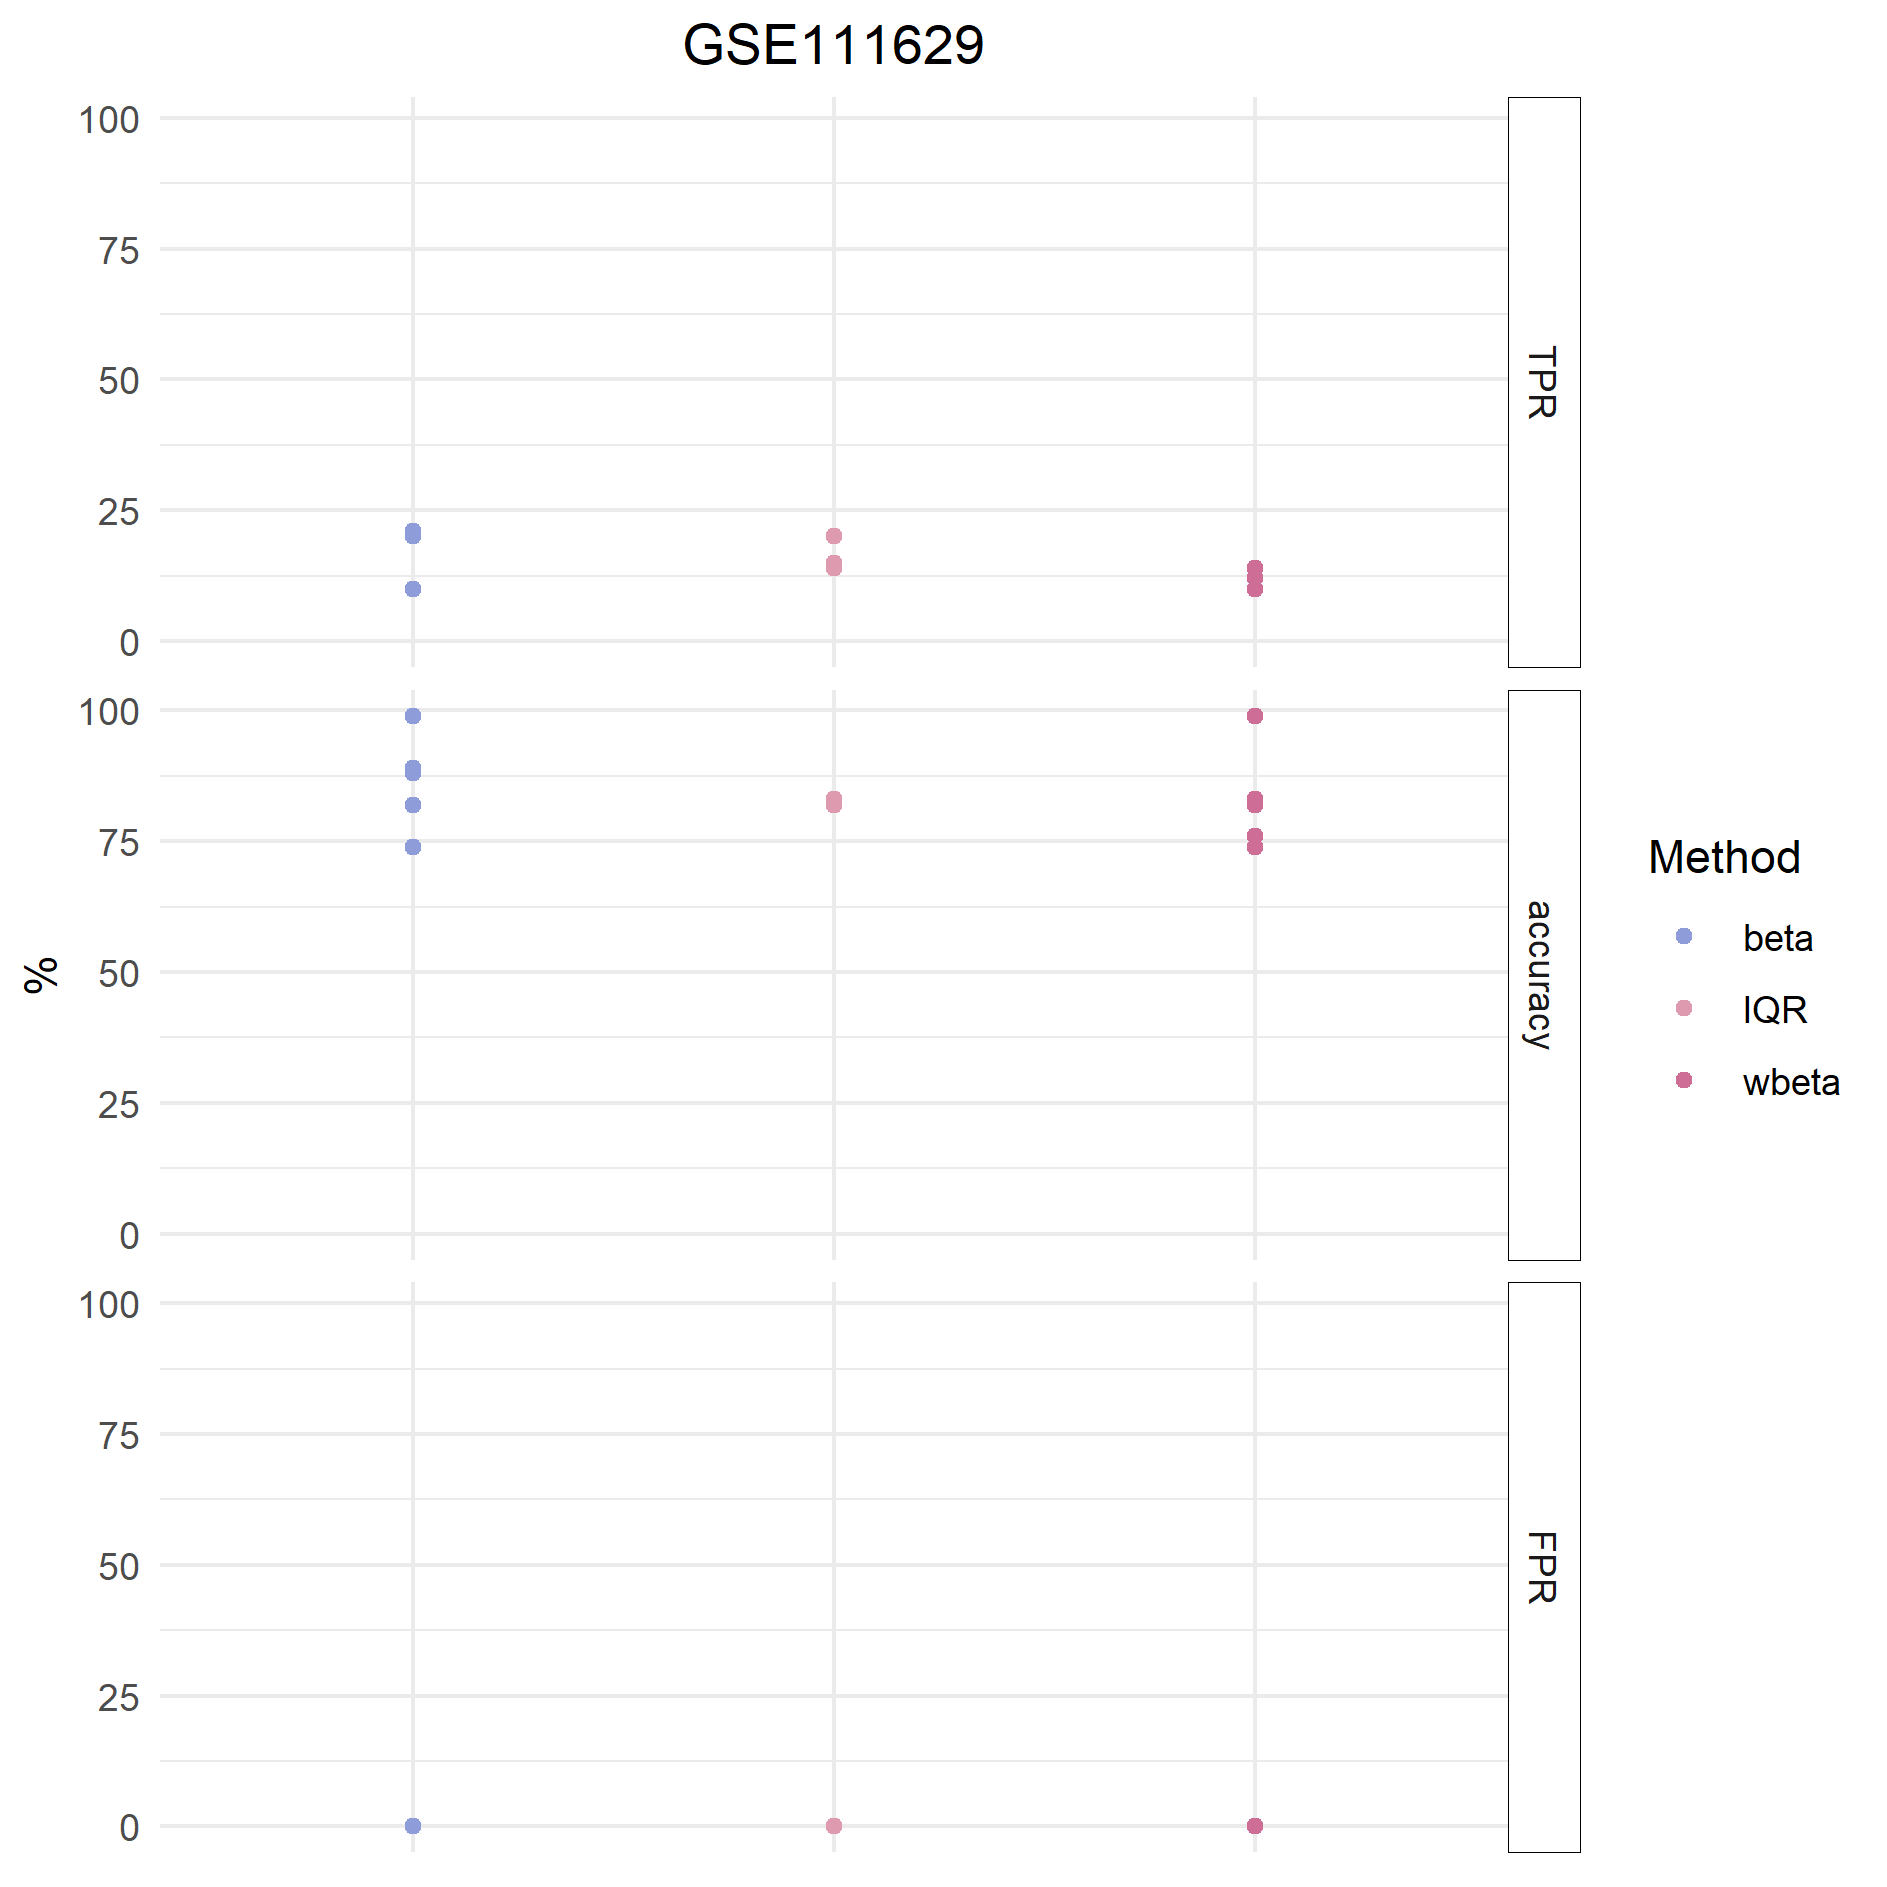
\includegraphics[width=27.99in]{C:/Users/nla94/Documents/GitHub/Supplementary-Material/Abarrategui_2021/result_files/4-Graph/GSE111629_chr5_67583971_67584381} 

}

\caption{epimutations performance using GSE111629 cohort to detect the epivariation located in chr5:67583971-67584381}\label{fig:graph_GSE111629_2}
\end{figure}

\begin{figure}

{\centering 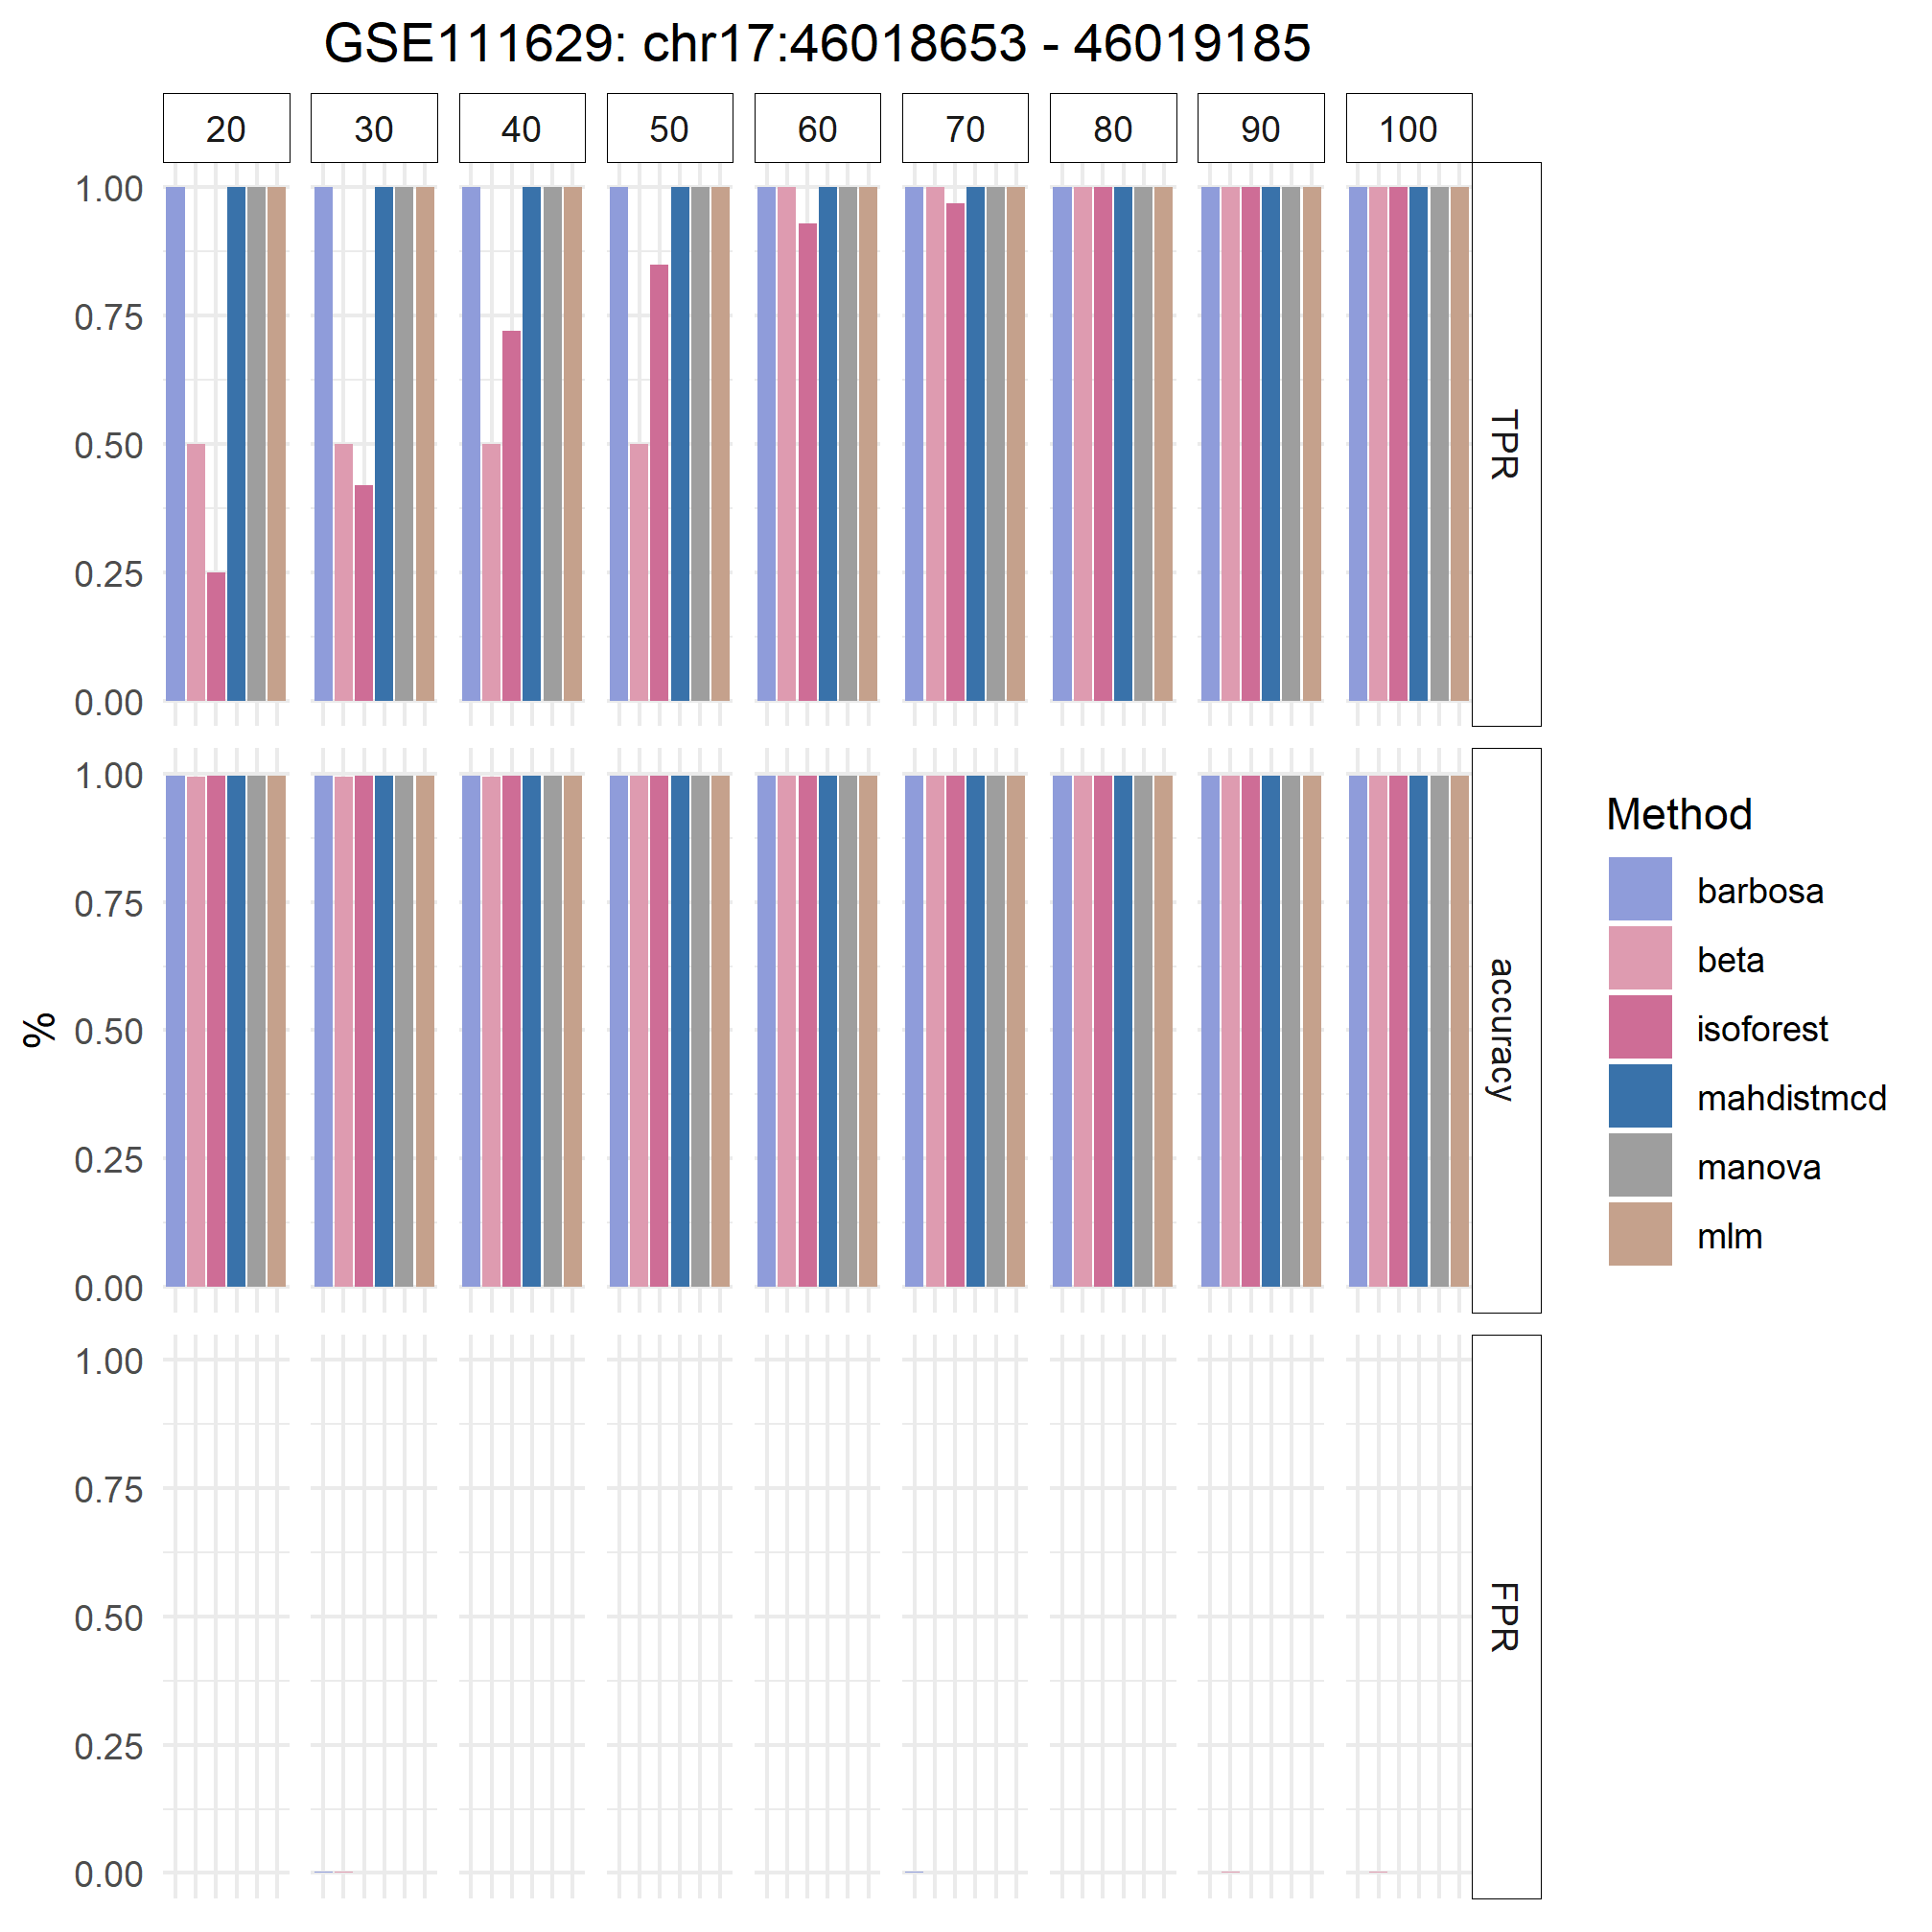
\includegraphics[width=27.99in]{C:/Users/nla94/Documents/GitHub/Supplementary-Material/Abarrategui_2021/result_files/4-Graph/GSE111629_chr17_46018653_46019185} 

}

\caption{epimutations performance using GSE111629 cohort to detect the epivariation located in chr17:46018653-46019185}\label{fig:graph_GSE111629_3}
\end{figure}

\begin{figure}

{\centering 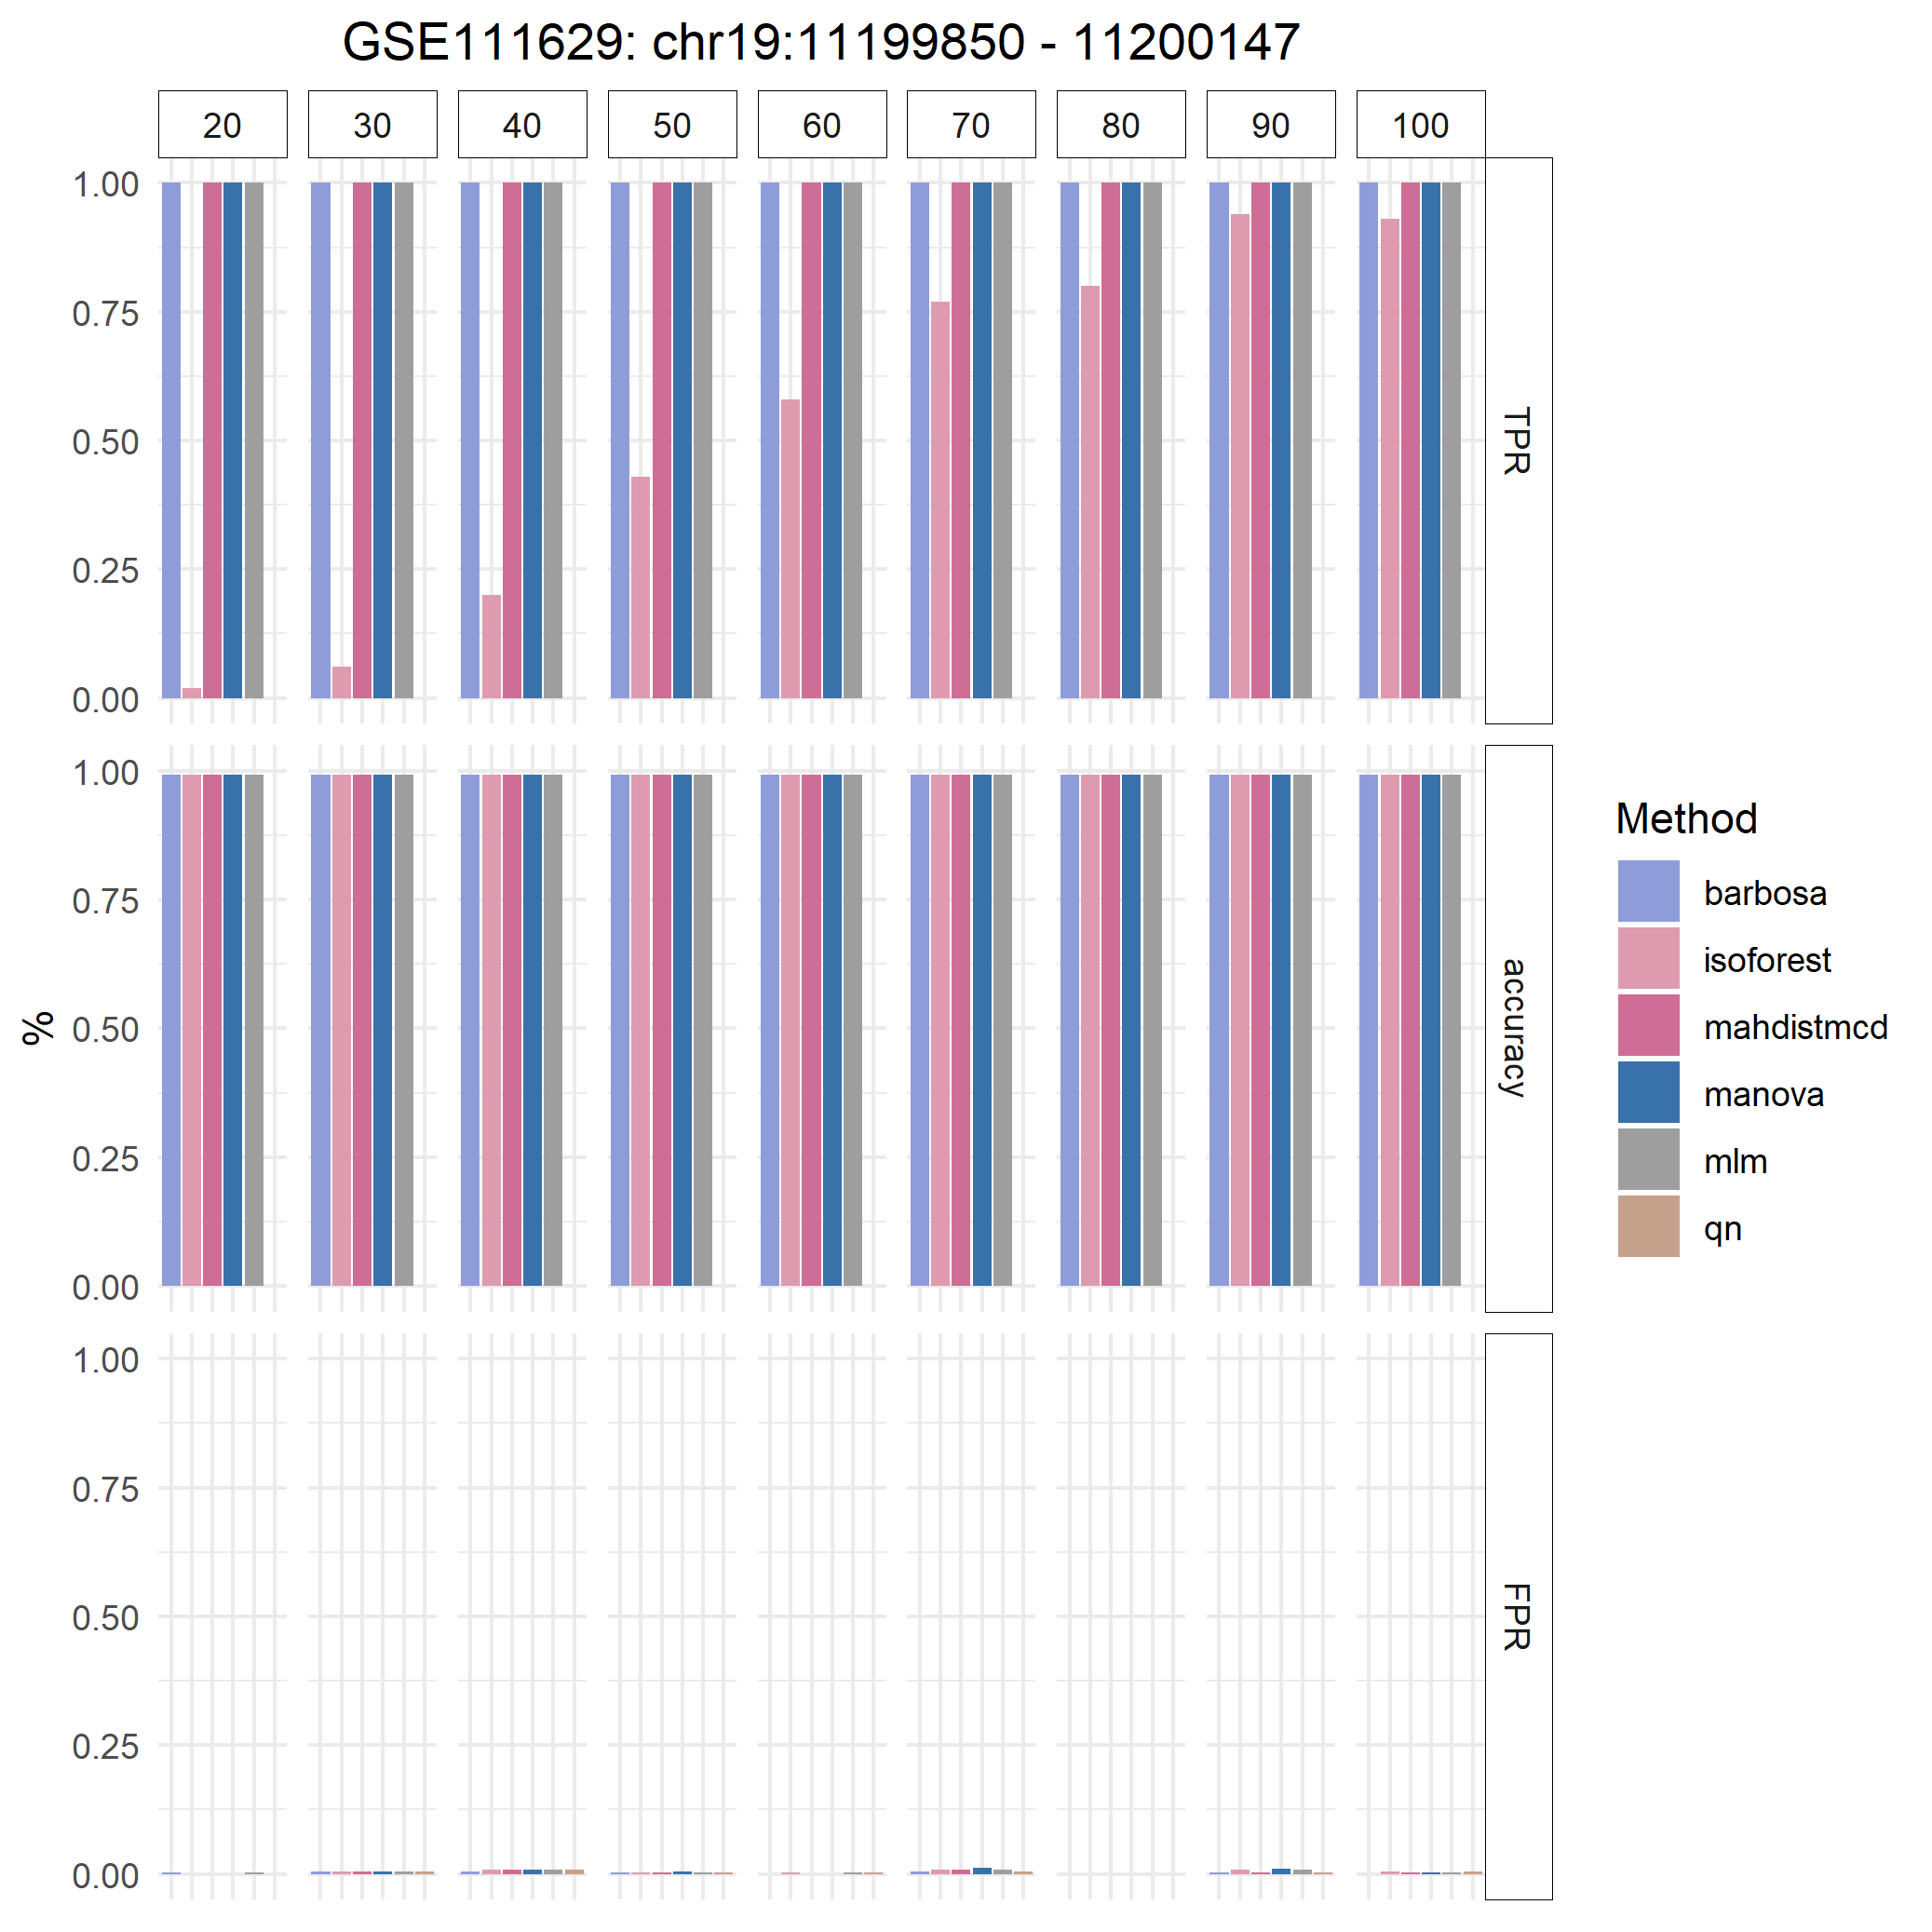
\includegraphics[width=27.99in]{C:/Users/nla94/Documents/GitHub/Supplementary-Material/Abarrategui_2021/result_files/4-Graph/GSE111629_chr19_11199850_11200147} 

}

\caption{epimutations performance using GSE111629 cohort to detect the epivariation located in chr5:11199850-11200147}\label{fig:graph_GSE111629_4}
\end{figure}

\newpage

\hypertarget{acknowledgements}{%
\section{Acknowledgements}\label{acknowledgements}}

We acknowledge the organizers of the
\href{https://www.biohackathon-europe.org/}{European BioHackathon 2020}
for their support.

All the team members of \emph{Project \#5} for the contribution to this
package:

\begin{longtable}[]{@{}llcll@{}}
\toprule
\begin{minipage}[b]{0.13\columnwidth}\raggedright
Name\strut
\end{minipage} & \begin{minipage}[b]{0.19\columnwidth}\raggedright
Surname\strut
\end{minipage} & \begin{minipage}[b]{0.15\columnwidth}\centering
ORCID\strut
\end{minipage} & \begin{minipage}[b]{0.27\columnwidth}\raggedright
Affiliation\strut
\end{minipage} & \begin{minipage}[b]{0.13\columnwidth}\raggedright
Team\strut
\end{minipage}\tabularnewline
\midrule
\endhead
\begin{minipage}[t]{0.13\columnwidth}\raggedright
Leire\strut
\end{minipage} & \begin{minipage}[t]{0.19\columnwidth}\raggedright
Abarrategui\strut
\end{minipage} & \begin{minipage}[t]{0.15\columnwidth}\centering
0000-0002-1175-038X\strut
\end{minipage} & \begin{minipage}[t]{0.27\columnwidth}\raggedright
Faculty of Medical Sciences, Newcastle University, Newcastle-Upon-Tyne,
UK; Autonomous University of Barcelona (UAB), Barcelona, Spain\strut
\end{minipage} & \begin{minipage}[t]{0.13\columnwidth}\raggedright
Development\strut
\end{minipage}\tabularnewline
\begin{minipage}[t]{0.13\columnwidth}\raggedright
Lordstrong\strut
\end{minipage} & \begin{minipage}[t]{0.19\columnwidth}\raggedright
Akano\strut
\end{minipage} & \begin{minipage}[t]{0.15\columnwidth}\centering
0000-0002-1404-0295\strut
\end{minipage} & \begin{minipage}[t]{0.27\columnwidth}\raggedright
College of Medicine, University of Ibadan\strut
\end{minipage} & \begin{minipage}[t]{0.13\columnwidth}\raggedright
Development\strut
\end{minipage}\tabularnewline
\begin{minipage}[t]{0.13\columnwidth}\raggedright
James\strut
\end{minipage} & \begin{minipage}[t]{0.19\columnwidth}\raggedright
Baye\strut
\end{minipage} & \begin{minipage}[t]{0.15\columnwidth}\centering
0000-0002-0078-3688\strut
\end{minipage} & \begin{minipage}[t]{0.27\columnwidth}\raggedright
Wellcome/MRC Cambridge Stem Cell Institute, University of Cambridge,
Cambridge CB2 0AW, UK; Department of Physics, University of Cambridge,
Cambridge CB2 3DY, UK\strut
\end{minipage} & \begin{minipage}[t]{0.13\columnwidth}\raggedright
Development\strut
\end{minipage}\tabularnewline
\begin{minipage}[t]{0.13\columnwidth}\raggedright
Alejandro\strut
\end{minipage} & \begin{minipage}[t]{0.19\columnwidth}\raggedright
Caceres\strut
\end{minipage} & \begin{minipage}[t]{0.15\columnwidth}\centering
-\strut
\end{minipage} & \begin{minipage}[t]{0.27\columnwidth}\raggedright
ISGlobal, Barcelona Institute for Global Health, Dr Aiguader 88, 08003
Barcelona, Spain; Centro de Investigación Biomédica en Red en
Epidemiología y Salud Pública (CIBERESP), Madrid, Spain\strut
\end{minipage} & \begin{minipage}[t]{0.13\columnwidth}\raggedright
Development\strut
\end{minipage}\tabularnewline
\begin{minipage}[t]{0.13\columnwidth}\raggedright
Carles\strut
\end{minipage} & \begin{minipage}[t]{0.19\columnwidth}\raggedright
Hernandez-Ferrer\strut
\end{minipage} & \begin{minipage}[t]{0.15\columnwidth}\centering
0000-0002-8029-7160\strut
\end{minipage} & \begin{minipage}[t]{0.27\columnwidth}\raggedright
Centro Nacional de Análisis Genómico (CNAG-CRG), Center for Genomic,
Regulation; Barcelona Institute of Science and Technology (BIST),
Barcelona, Catalonia, Spain\strut
\end{minipage} & \begin{minipage}[t]{0.13\columnwidth}\raggedright
Development\strut
\end{minipage}\tabularnewline
\begin{minipage}[t]{0.13\columnwidth}\raggedright
Pavlo\strut
\end{minipage} & \begin{minipage}[t]{0.19\columnwidth}\raggedright
Hrab\strut
\end{minipage} & \begin{minipage}[t]{0.15\columnwidth}\centering
0000-0002-0742-8478\strut
\end{minipage} & \begin{minipage}[t]{0.27\columnwidth}\raggedright
Department of Genetics and Biotechnology, Biology faculty, Ivan Franko
National University of Lviv\strut
\end{minipage} & \begin{minipage}[t]{0.13\columnwidth}\raggedright
Validation\strut
\end{minipage}\tabularnewline
\begin{minipage}[t]{0.13\columnwidth}\raggedright
Raquel\strut
\end{minipage} & \begin{minipage}[t]{0.19\columnwidth}\raggedright
Manzano\strut
\end{minipage} & \begin{minipage}[t]{0.15\columnwidth}\centering
0000-0002-5124-8992\strut
\end{minipage} & \begin{minipage}[t]{0.27\columnwidth}\raggedright
Cancer Research UK Cambridge Institute; University of Cambridge,
Cambridge, United Kingdom\strut
\end{minipage} & \begin{minipage}[t]{0.13\columnwidth}\raggedright
Reporting\strut
\end{minipage}\tabularnewline
\begin{minipage}[t]{0.13\columnwidth}\raggedright
Margherita\strut
\end{minipage} & \begin{minipage}[t]{0.19\columnwidth}\raggedright
Mutarelli\strut
\end{minipage} & \begin{minipage}[t]{0.15\columnwidth}\centering
0000-0002-2168-5059\strut
\end{minipage} & \begin{minipage}[t]{0.27\columnwidth}\raggedright
Institute of Applied Sciences and Intelligent Systems (ISASI-CNR)\strut
\end{minipage} & \begin{minipage}[t]{0.13\columnwidth}\raggedright
Validation\strut
\end{minipage}\tabularnewline
\begin{minipage}[t]{0.13\columnwidth}\raggedright
Carlos\strut
\end{minipage} & \begin{minipage}[t]{0.19\columnwidth}\raggedright
Ruiz-Arenas\strut
\end{minipage} & \begin{minipage}[t]{0.15\columnwidth}\centering
0000-0002-6014-3498\strut
\end{minipage} & \begin{minipage}[t]{0.27\columnwidth}\raggedright
Centro de Investigación Biomédica en Red de Enfermedades Raras
(CIBERER), Barcelona, Spain; Universitat Pompeu Fabra (UPF), Barcelona,
Spain\strut
\end{minipage} & \begin{minipage}[t]{0.13\columnwidth}\raggedright
Reporting\strut
\end{minipage}\tabularnewline
\bottomrule
\end{longtable}

\hypertarget{references}{%
\section*{References}\label{references}}
\addcontentsline{toc}{section}{References}

\hypertarget{refs}{}
\leavevmode\hypertarget{ref-aref2019}{}%
Aref-Eshghi, Erfan, Eric G. Bend, Samantha Colaiacovo, Michelle Caudle,
Rana Chakrabarti, Melanie Napier, Lauren Brick, et al. 2019.
``Diagnostic Utility of Genome-Wide Dna Methylation Testing in
Genetically Unsolved Individuals with Suspected Hereditary Conditions.''
\emph{The American Journal of Human Genetics}.
\url{https://doi.org/https://doi.org/10.1016/j.ajhg.2019.03.008}.

\leavevmode\hypertarget{ref-cortes2021package}{}%
Cortes, David, and Maintainer David Cortes. 2021. ``Package `Isotree'.''

\leavevmode\hypertarget{ref-EU_RD}{}%
European-Commission. 2020. ``EU Research on Rare Diseases.''
\url{https://ec.europa.eu/info/research-and-innovation/research-area/health-research-and-innovation/rare-diseases_en}.

\leavevmode\hypertarget{ref-friedrich2017package}{}%
Friedrich, Sarah, Frank Konietschke, Markus Pauly, and Maintainer Sarah
Friedrich. 2017. ``Package `Manova. RM'.''

\leavevmode\hypertarget{ref-garg2020survey}{}%
Garg, Paras, Bharati Jadhav, Oscar L Rodriguez, Nihir Patel, Alejandro
Martin-Trujillo, Miten Jain, Sofie Metsu, et al. 2020. ``A Survey of
Rare Epigenetic Variation in 23,116 Human Genomes Identifies
Disease-Relevant Epivariations and Cgg Expansions.'' \emph{The American
Journal of Human Genetics} 107 (4): 654--69.

\leavevmode\hypertarget{ref-jaffe2012bump}{}%
Jaffe, Andrew E, Peter Murakami, Hwajin Lee, Jeffrey T Leek, M Daniele
Fallin, Andrew P Feinberg, and Rafael A Irizarry. 2012. ``Bump Hunting
to Identify Differentially Methylated Regions in Epigenetic Epidemiology
Studies.'' \emph{International Journal of Epidemiology} 41 (1):
200--209.

\leavevmode\hypertarget{ref-lionel2018improved}{}%
Lionel, Anath C, Gregory Costain, Nasim Monfared, Susan Walker, Miriam S
Reuter, S Mohsen Hosseini, Bhooma Thiruvahindrapuram, et al. 2018.
``Improved Diagnostic Yield Compared with Targeted Gene Sequencing
Panels Suggests a Role for Whole-Genome Sequencing as a First-Tier
Genetic Test.'' \emph{Genetics in Medicine} 20 (4): 435--43.

\leavevmode\hypertarget{ref-lopez2016social}{}%
López-Bastida, Julio, Juan Oliva-Moreno, Renata Linertová, and Pedro
Serrano-Aguilar. 2016. ``Social/Economic Costs and Health-Related
Quality of Life in Patients with Rare Diseases in Europe.'' Springer.

\leavevmode\hypertarget{ref-barbosa2018}{}%
M, Barbosa, Joshi RS, Garg R, Martin-Trujillo A, Patel N, Jadhav B,
Watson CT, et al. 2018. ``Identification of Rare de Novo Epigenetic
Variations in Congenital Disorders.'' \emph{Nature Communications}.
\url{https://doi.org/https://doi.org/10.1038/s41467-018-04540-x}.

\leavevmode\hypertarget{ref-maechler2021package}{}%
Maechler, Martin, Peter Rousseeuw, Christophe Croux, Valentin Todorov,
Andreas Ruckstuhl, Matias Salibian-Barrera, Tobias Verbeke, Manuel
Koller, Eduardo LT Conceicao, and Maria Anna di Palma. 2021. ``Package
`Robustbase'.'' \emph{Basic Robust Statistics}.

\leavevmode\hypertarget{ref-martin2020multivariate}{}%
Martı́n, Diego Garrido. 2020. ``A Multivariate Approach to Study the
Genetic Determinants of Phenotypic Traits.'' PhD thesis, Universitat
Pompeu Fabra.

\leavevmode\hypertarget{ref-serra2015dna}{}%
Serra-Juhé, Clara, Ivon Cuscó, Aı̈da Homs, Raquel Flores, Núria Torán,
and Luis A Pérez-Jurado. 2015. ``DNA Methylation Abnormalities in
Congenital Heart Disease.'' \emph{Epigenetics} 10 (2): 167--77.

\end{document}
